% Unofficial University of Cambridge Poster Template
% https://github.com/andiac/gemini-cam
% a fork of https://github.com/anishathalye/gemini
% also refer to https://github.com/k4rtik/uchicago-poster

\documentclass[final]{beamer}

% ====================
% Packages
% ====================

\usepackage[T1]{fontenc}
\usepackage{lmodern}
\usepackage[orientation=portrait,size=a1,scale=1.15]{beamerposter}
\usetheme{gemini}
\usecolortheme{nott}
\usepackage{graphicx}
\usepackage{booktabs}
\usepackage{tikz}
\usepackage{pgfplots}
\pgfplotsset{compat=1.14}
\usepackage{anyfontsize}
\usepackage{subcaption} % для subfigure
\usepackage[table]{xcolor}
\usepackage[table]{xcolor}
% \definecolor{mycolor1}{HTML}{dde9c7}
\definecolor{mycolor1}{HTML}{c1d796}


% ====================
% Lengths
% ====================

% If you have N columns, choose \sepwidth and \colwidth such that
% (N+1)*\sepwidth + N*\colwidth = \paperwidth
\newlength{\sepwidth}
\newlength{\colwidth}
\setlength{\sepwidth}{0.025\paperwidth}
\setlength{\colwidth}{0.45\paperwidth}

\newcommand{\separatorcolumn}{\begin{column}{\sepwidth}\end{column}}
\renewcommand{\figurename}{Рис.}
\renewcommand{\tablename}{Табл.}

% ====================
% Title
% ====================

\title{РАЗРАБОТКА МЕТОДА ОЦЕНКИ НАЛИЧИЯ ЗАКОНОМЕРНОСТЕЙ В
ПРОСТРАНСТВЕННОЙ ОРГАНИЗАЦИИ ДЕНДРИТА НЕЙРОНА}

\author{Е.К. Липс \inst{1} \and Д.С. Смирнова \inst{2} \and Е.И. Пчицкая \inst{2} \and В.С. Чуканов \inst{1,2}}

\institute[shortinst]{\inst{1} Кафедра прикладной математики, Санкт-Петербургский политехнический университет  \samelineand \\
\inst{2} Лаборатория анализа биомедицинских изображений и данных,
Санкт-Петербургский политехнический университет 
}

% ====================
% Footer (optional)
% ====================

\footercontent{
  \href{ }{ } \hfill
  Неделя Науки ФИЗМЕХ 2025 \hfill
  \href{ }{ }}
% (can be left out to remove footer)


% ====================
% Logo (optional)
% ====================

% use this to include logos on the left and/or right side of the header:
% \logoright{
\includegraphics[height=2.5cm]{logos/utfpr-logo.png}}
% \logoleft{\hspace{20ex}
\includegraphics[height=3.5cm]{logos/ppgca-logo.png}}

% ====================
% Body
% ====================

\begin{document}

% Refer to https://github.com/k4rtik/uchicago-poster
% logo: https://www.cam.ac.uk/brand-resources/about-the-logo/logo-downloads
% \addtobeamertemplate{headline}{}
% {
%     \begin{tikzpicture}[remember picture,overlay]
%       \node [anchor=north west, inner sep=3cm] at ([xshift=-2.5cm,yshift=1.75cm]current page.north west)
%       {\includegraphics[height=7cm]{logos/unott-logo.eps}}; 
%     \end{tikzpicture}
% }

\begin{frame}[t]
\begin{columns}[t]
\separatorcolumn

\begin{column}{\colwidth}

  \begin{block}{Цели}
    % Современные исследования, направленные на изучение организации нейронных сетей при нейропсихиатрических заболеваниях, свидетельствуют о ключевом значении структурных изменений шипиковых синапсов в патогенезе данных заболеваний. Было выявлено, что взаимное расположение шипов и степень их сгруппированности напрямую связаны с эффективностью обработки и хранения информации в нейронных сетях. \\ 
    % Данная работа направлена на разработку методов оценки сгруппированности дендритных шипиков и выявление закономерностей взаимного расположения шипиков на дендрите в норме и при нейропатологии.
    % Цели данной работы: 
    \begin{itemize}
        \item разработка методов оценки сгруппированности дендритных шипиков
        \item выявление закономерностей взаимного расположения шипиков на дендрите в норме и при нейропатологии.
    \end{itemize}

  \end{block}

  \begin{block}{Методы}

    % Nam vulputate nunc felis, non condimentum lacus porta ultrices. Nullam sed
    % sagittis metus. Etiam consectetur gravida urna quis suscipit.
    % \textbf{Предобработка данных} представлена на рис. 1.

    % \begin{figure}
    %     \centering
    %     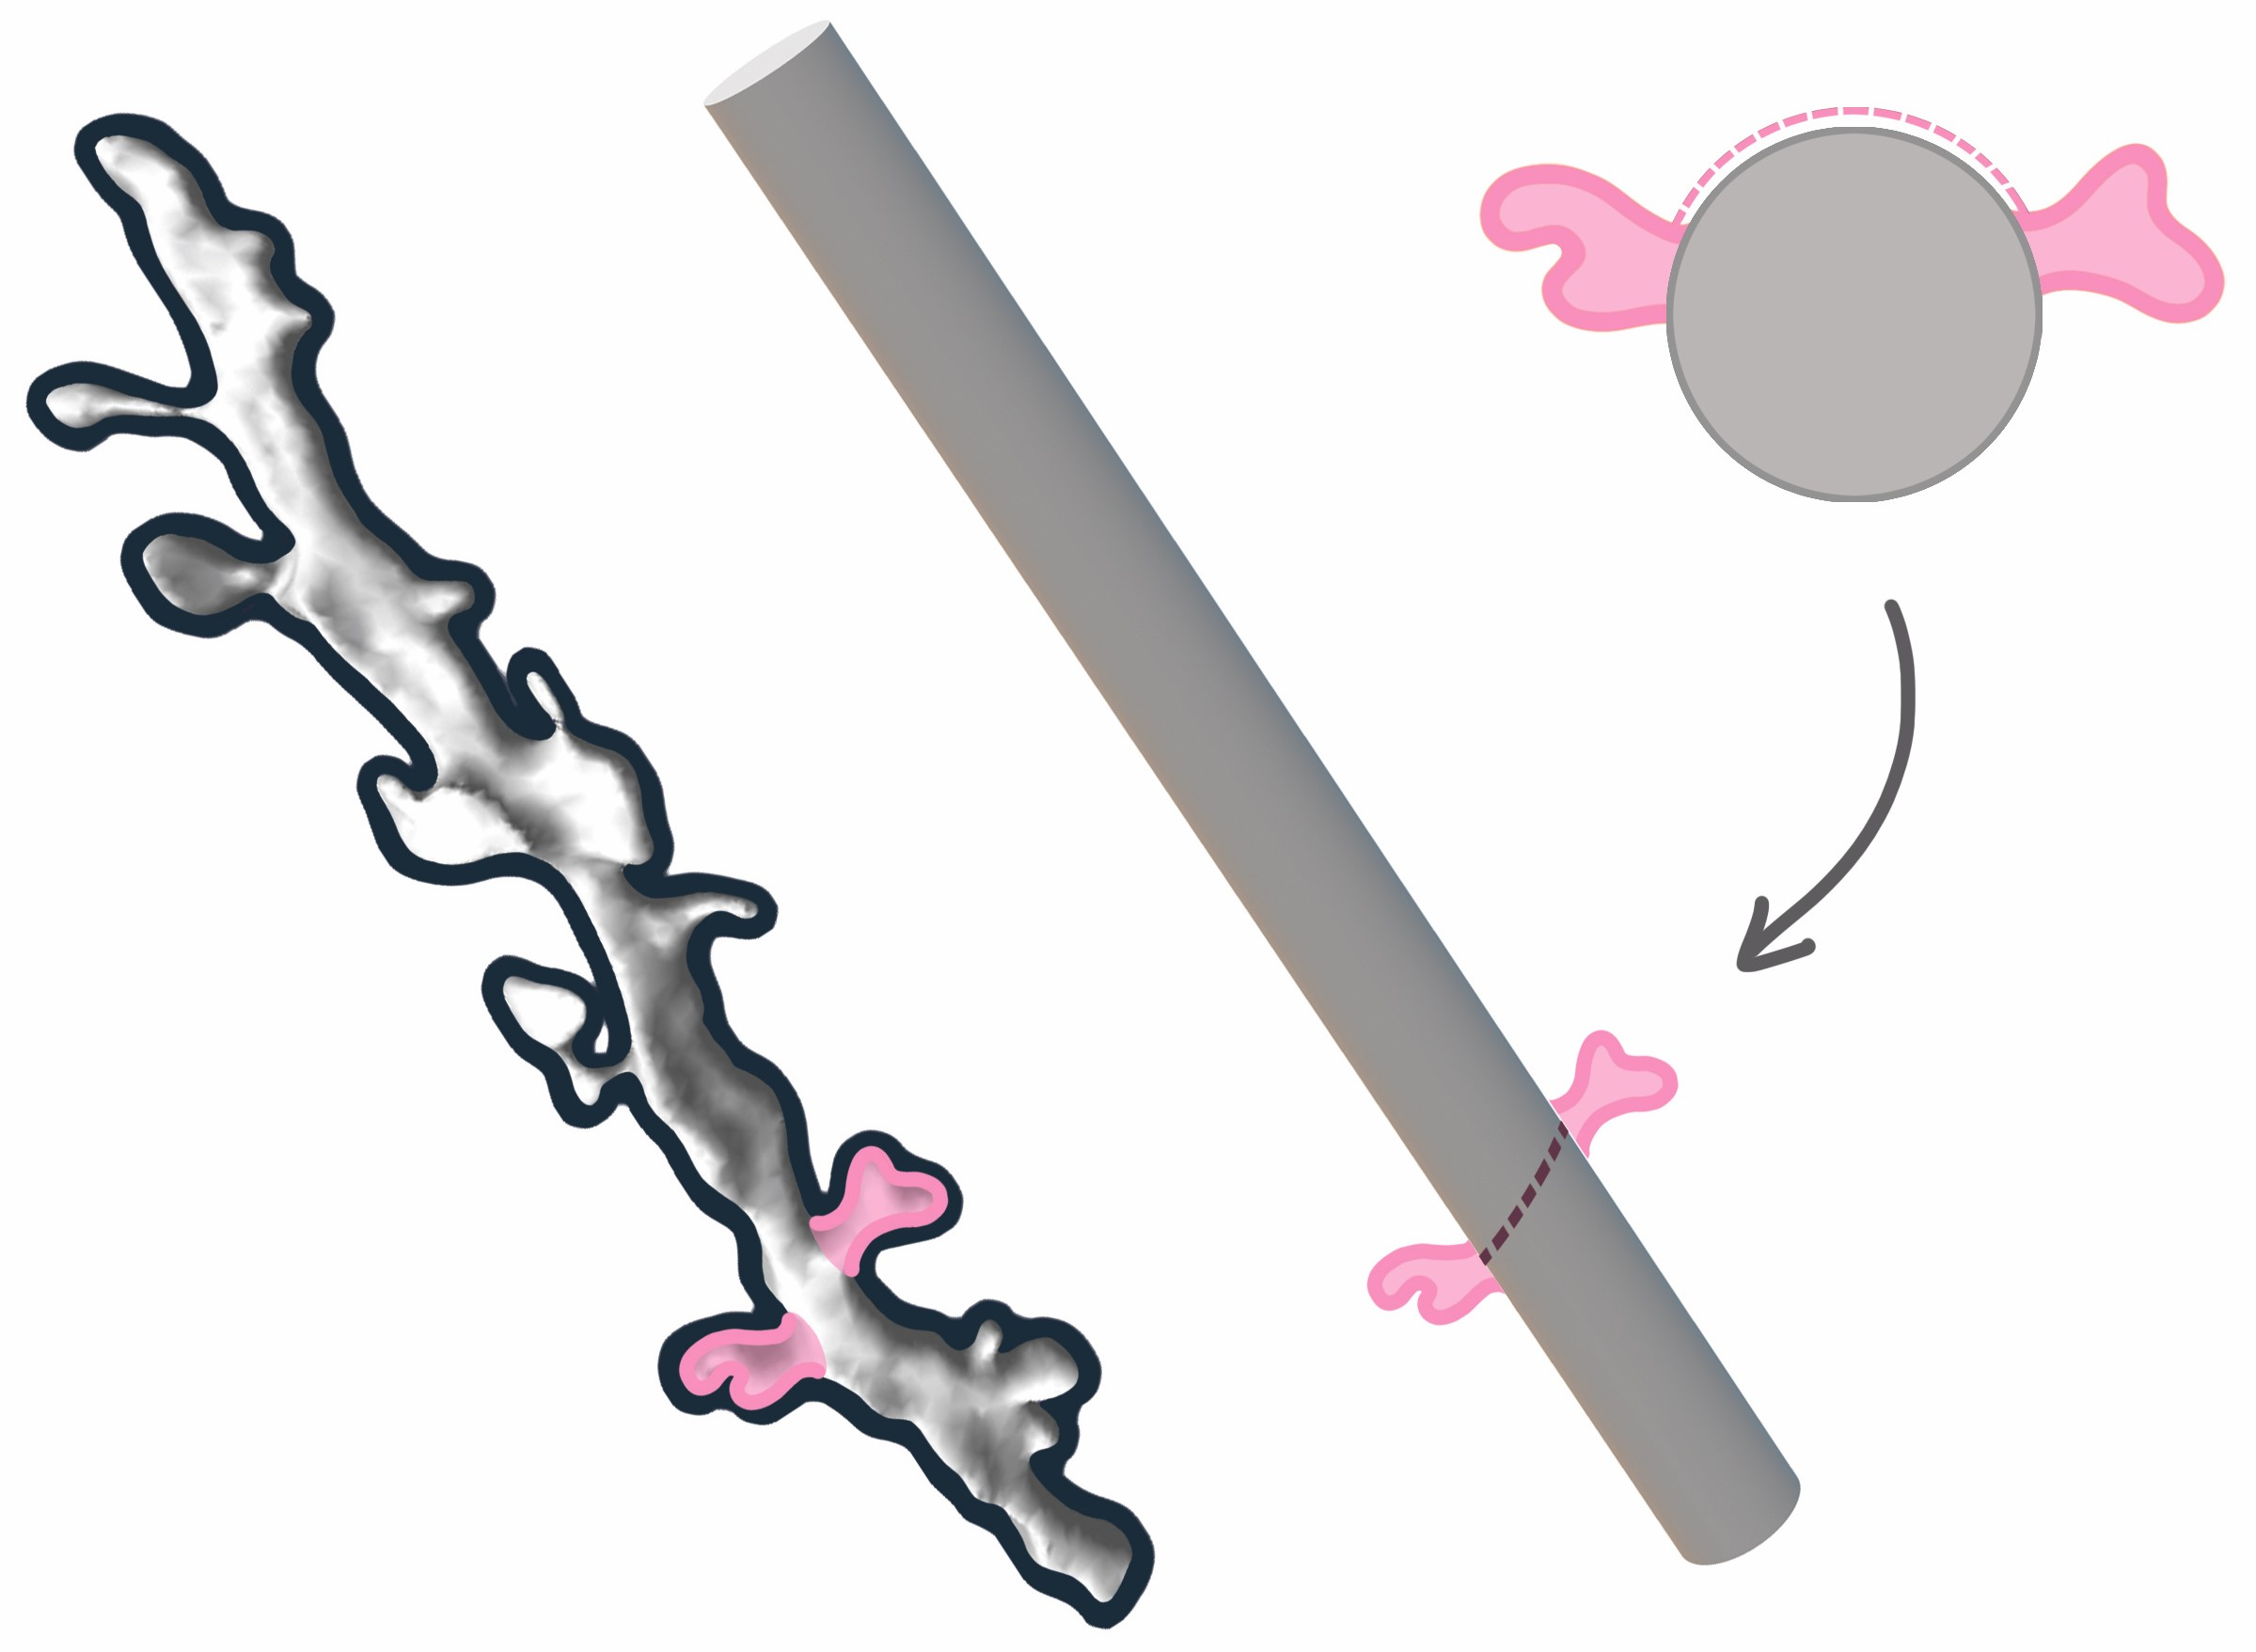
\includegraphics[width=0.5\linewidth]{цк.jpg}
    %     \caption{Переход в цилиндрические координаты}
    %     \label{fig:enter-label}
    % \end{figure}
    
    % \vspace{-0.7em}
    \heading{Анализ распределения попарных расстояний между шипиками:}
    Подсчет попарных расстояний между всеми дендритными шипиками, построение их распределения и вычисление описательных статистик. 
    \heading{Вычисление метрики NNdist: $ \; \; \; NNdist = \frac {1} {n} \sum\limits_{i=1}^n \min\limits_{i \neq j}⁡ dist(p_i,p_j ) $}
    % $$ NNdist = \frac {1} {n} \sum\limits_{i=1}^n \min\limits_{i \neq j}⁡ dist(p_i,p_j ) $$
    где $p_i$ – некоторая точка, $p_j$ – ближайший сосед $p_i$. 
    \heading{Вычисление функции парной корреляции PCF: $ \; \; \; g(r)= \frac {\rho(r)} {\rho_0} $} 
    где $\rho(r)$ – плотность точек на расстоянии $r$, $\rho_0$ – плотность точек.\\\\
    \vspace{0.5em} 
    PCF вычисляет вероятность нахождения точки на любом расстоянии от некоторой заданной точки, позволяя выявить наличие структуры в расположении точек.
    % $$g(r)= \frac {\rho(r)} {\rho_0} $$
    

    % \vspace{-0.3em} 
    \begin{figure}
        \centering
        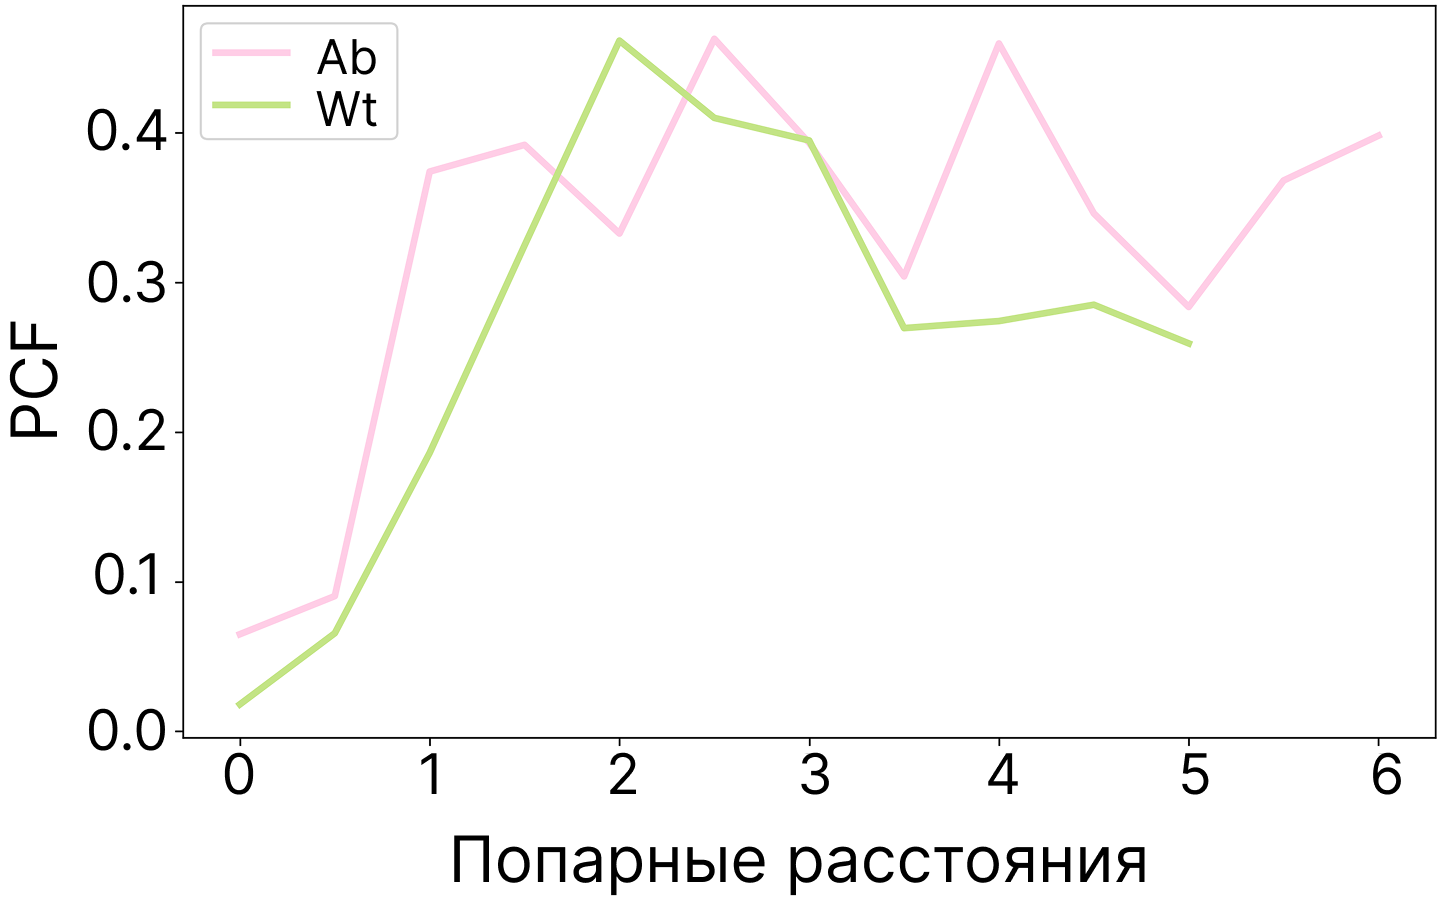
\includegraphics[width=0.5\linewidth]{pcf_figma.png}
        \caption{Пример построения графика PCF}
        \label{fig:enter-label}
    \end{figure}
    \vspace{-0.7em} 
    % \vspace{-0.7em}
    % \begin{figure}[ht]
    % \centering
    % \begin{minipage}[t]{0.48\textwidth}
    %     \centering
    %     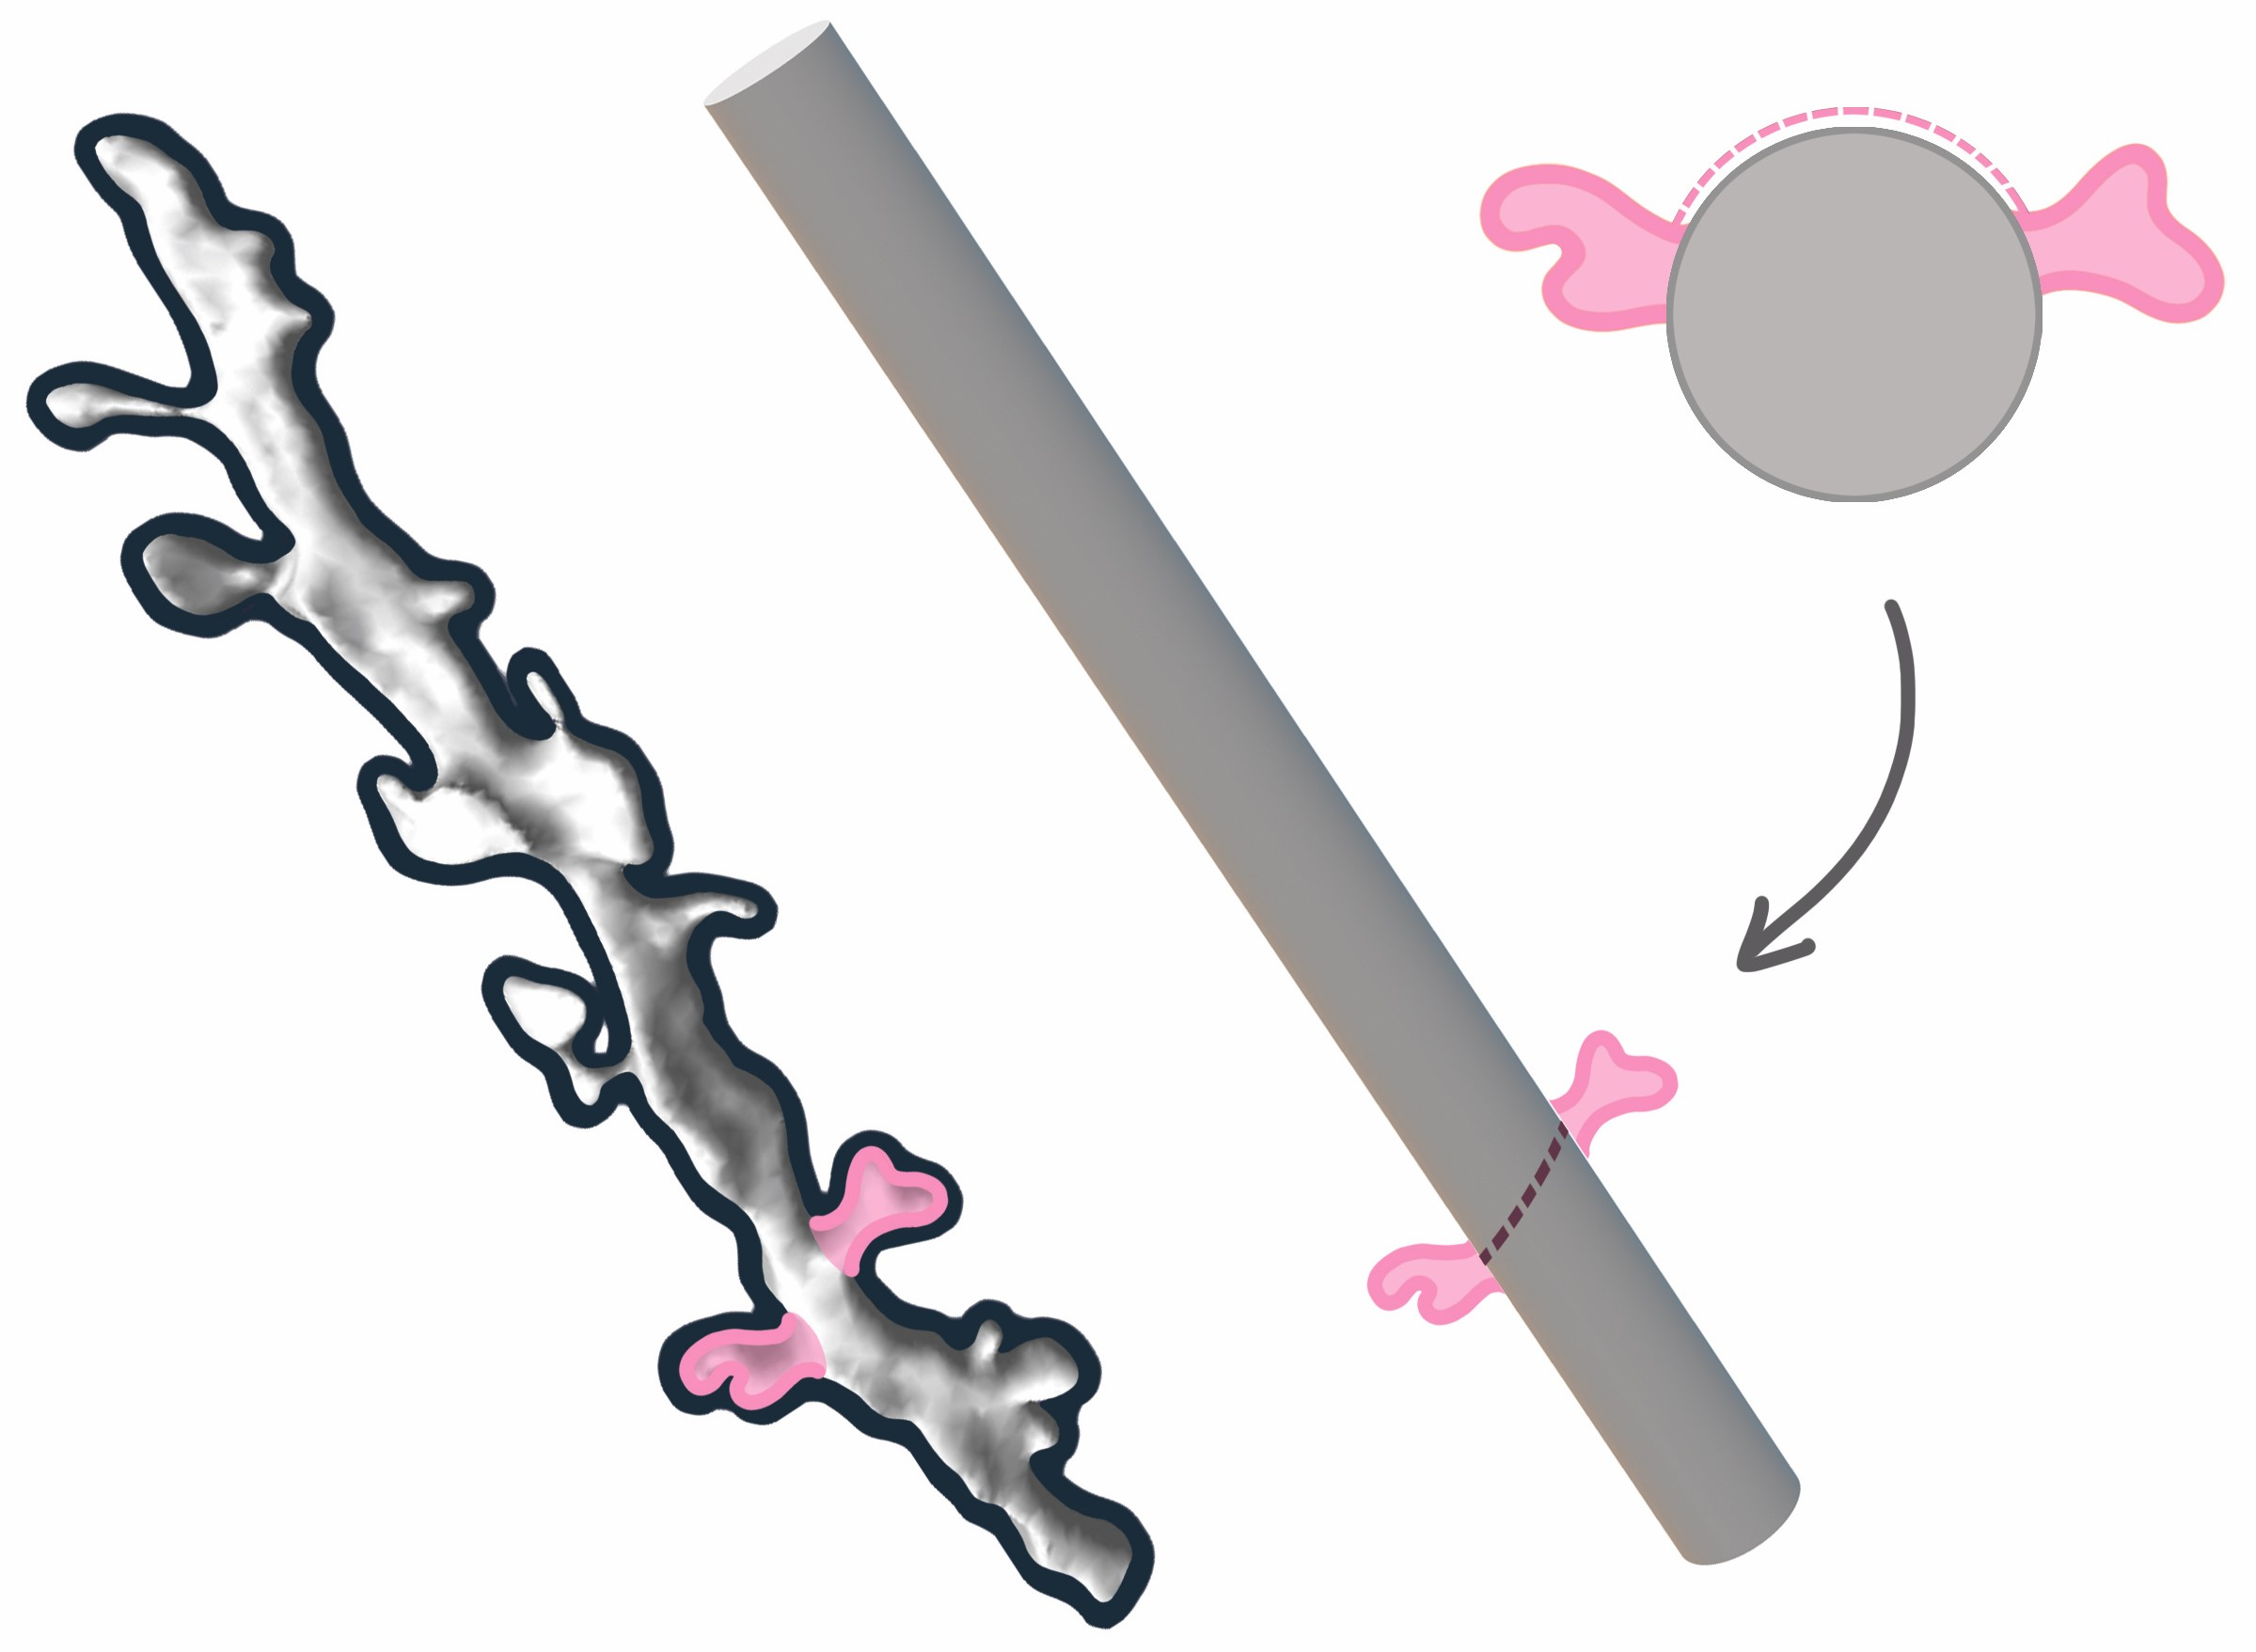
\includegraphics[width=\linewidth]{цк.jpg}
    %     \caption{\centering Вычисление расстояния в цилиндрических координатах}
    %     \label{fig:graph1}
    % \end{minipage}
    % \hfill
    % \begin{minipage}[t]{0.48\textwidth}
    %     \centering
    %     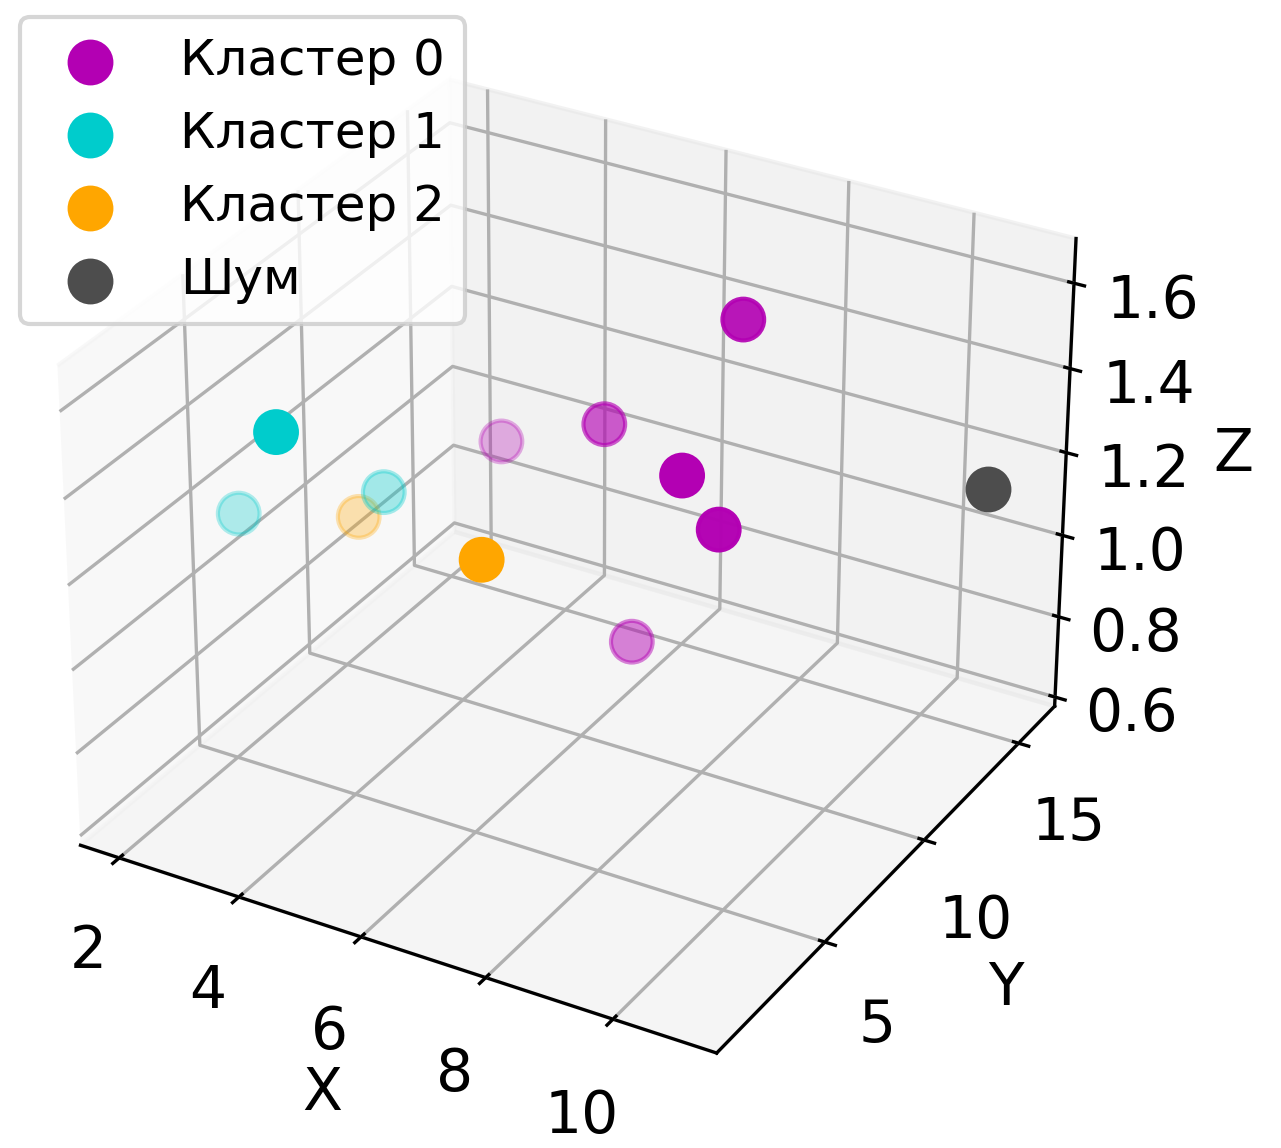
\includegraphics[width=\linewidth]{ab23-2_processed.png}
    %     \caption{Пример результата кластеризации}
    %     \label{fig:graph2}
    % \end{minipage}
    % \end{figure}
    \heading{Вычисление энтропии Шеннона для PCF: $ \; \; \; S= -\sum\limits_{i=1}^n p(r_i) \cdot \log⁡ p(r_i) $}
    Энтропия Шеннона позволяет количественно оценить степень упорядоченности или хаотичности в распределении точек системы.
    % Энтропия Шеннона была использована для количественной оценки графика PCF.  
    % , которая позволяет количественно оценить степень упорядоченности или хаотичности в распределении точек системы. 
    % $$ S= -\sum\limits_{i=1}^n p(r_i) \cdot \log⁡ p(r_i) $$
    \heading{Вычисление меры автокорреляции Морана: $ \; \; \; I= \frac {N} {W}  \cdot \sum\limits_{i=1}^n \sum\limits_{j=1}^n \frac {w_{ij} (x_i- \bar {x})(x_j  - \bar {x}) } {\sum\limits_{i=1}^n(x_i- \bar {x})^2 } $}
    % $$ I= \frac {N} {W}  \cdot \sum\limits_{i=1}^n \sum\limits_{j=1}^n \frac {w_{ij} (x_i- \bar {x})(x_j  - \bar {x}) } {\sum\limits_{i=1}^n(x_i- \bar {x})^2 } $$
    где $N$ – количество точек, $w_{ij}$ – вес связи между точками $i$ и $j$, $W$ – сумма всех весов $w_{ij}$, $x_i$, $x_j$ – значение метрики для точек $i$ и $j$, $\bar {x}$ – среднее значение метрики.
    \heading{Анализ пространственных кластеров}
    % Вид пространственной сгруппированности шипиков возможно оценить решением задачи кластеризации точек в физическом пространстве. \\
    % \vspace{0.8em}
    Метод кластеризации - DBSCAN с выбором радиуса окрестности точки ($\varepsilon$) и минимального количества точек в окрестности для создания кластера (m).
    % \vspace{-0.7em}
    % \begin{itemize}
    %     \item $\varepsilon$ - радиус окрестности точки
    %     \item min\_sampes (m) - минимальное количество точек в $\varepsilon$-окрестности для создания кластера.
    % \end{itemize}
    % \vspace{-0.7em}
    % \begin{figure}[ht]
    % \centering
    % \begin{subfigure}{ }
    %     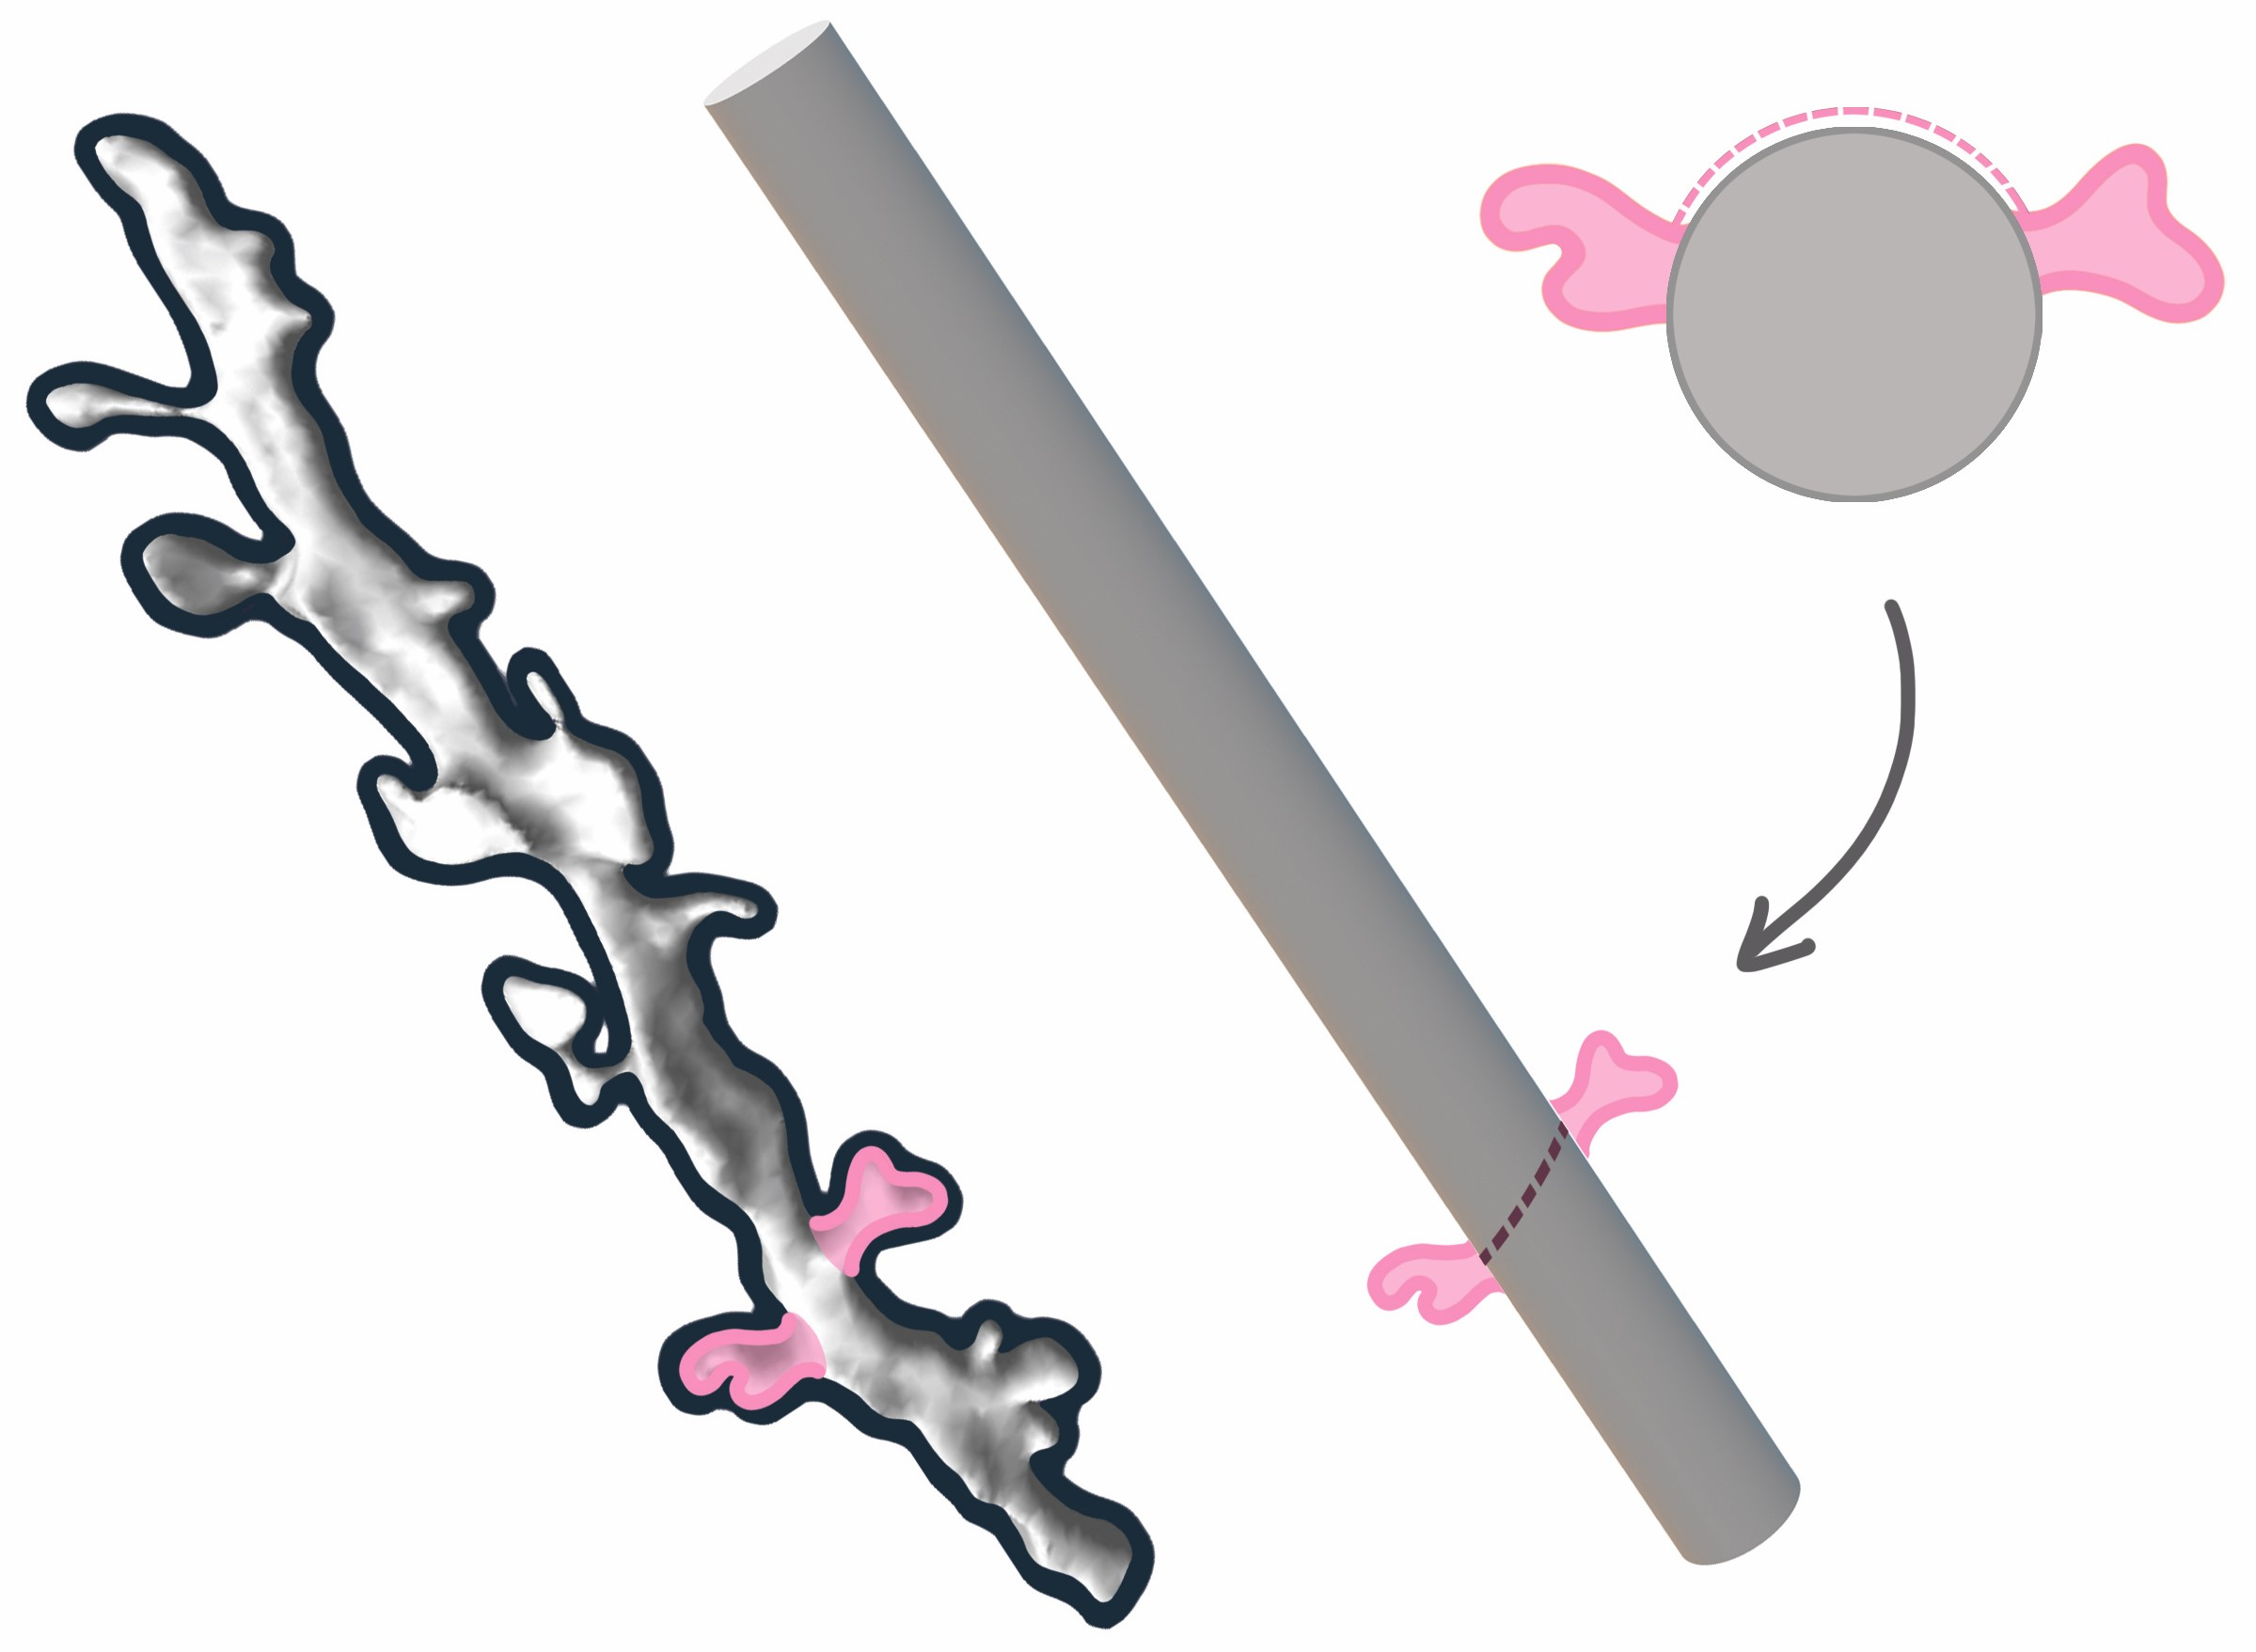
\includegraphics[width=\textwidth /4]{цк.jpg}
    %     \caption{Перевод в цк}
    %     \label{fig:graph1}
    % \end{subfigure}
    % % \hfill % заполняет пространство между графиками
    % \begin{subfigure}{ }
    %     \includegraphics[width=\textwidth/4]{graph2.png}
    %     \caption{Подпись }
    %     \label{fig:graph2}
    % \end{subfigure}
    % % \caption{Общая подпись для обоих графиков (опционально)}
    % \label{fig:both}
    % \end{figure}


    % \begin{figure}[ht]
    %     \centering
    %     \begin{subfigure}[b]{0.48\textwidth} % задаем ширину подрисунка
    %         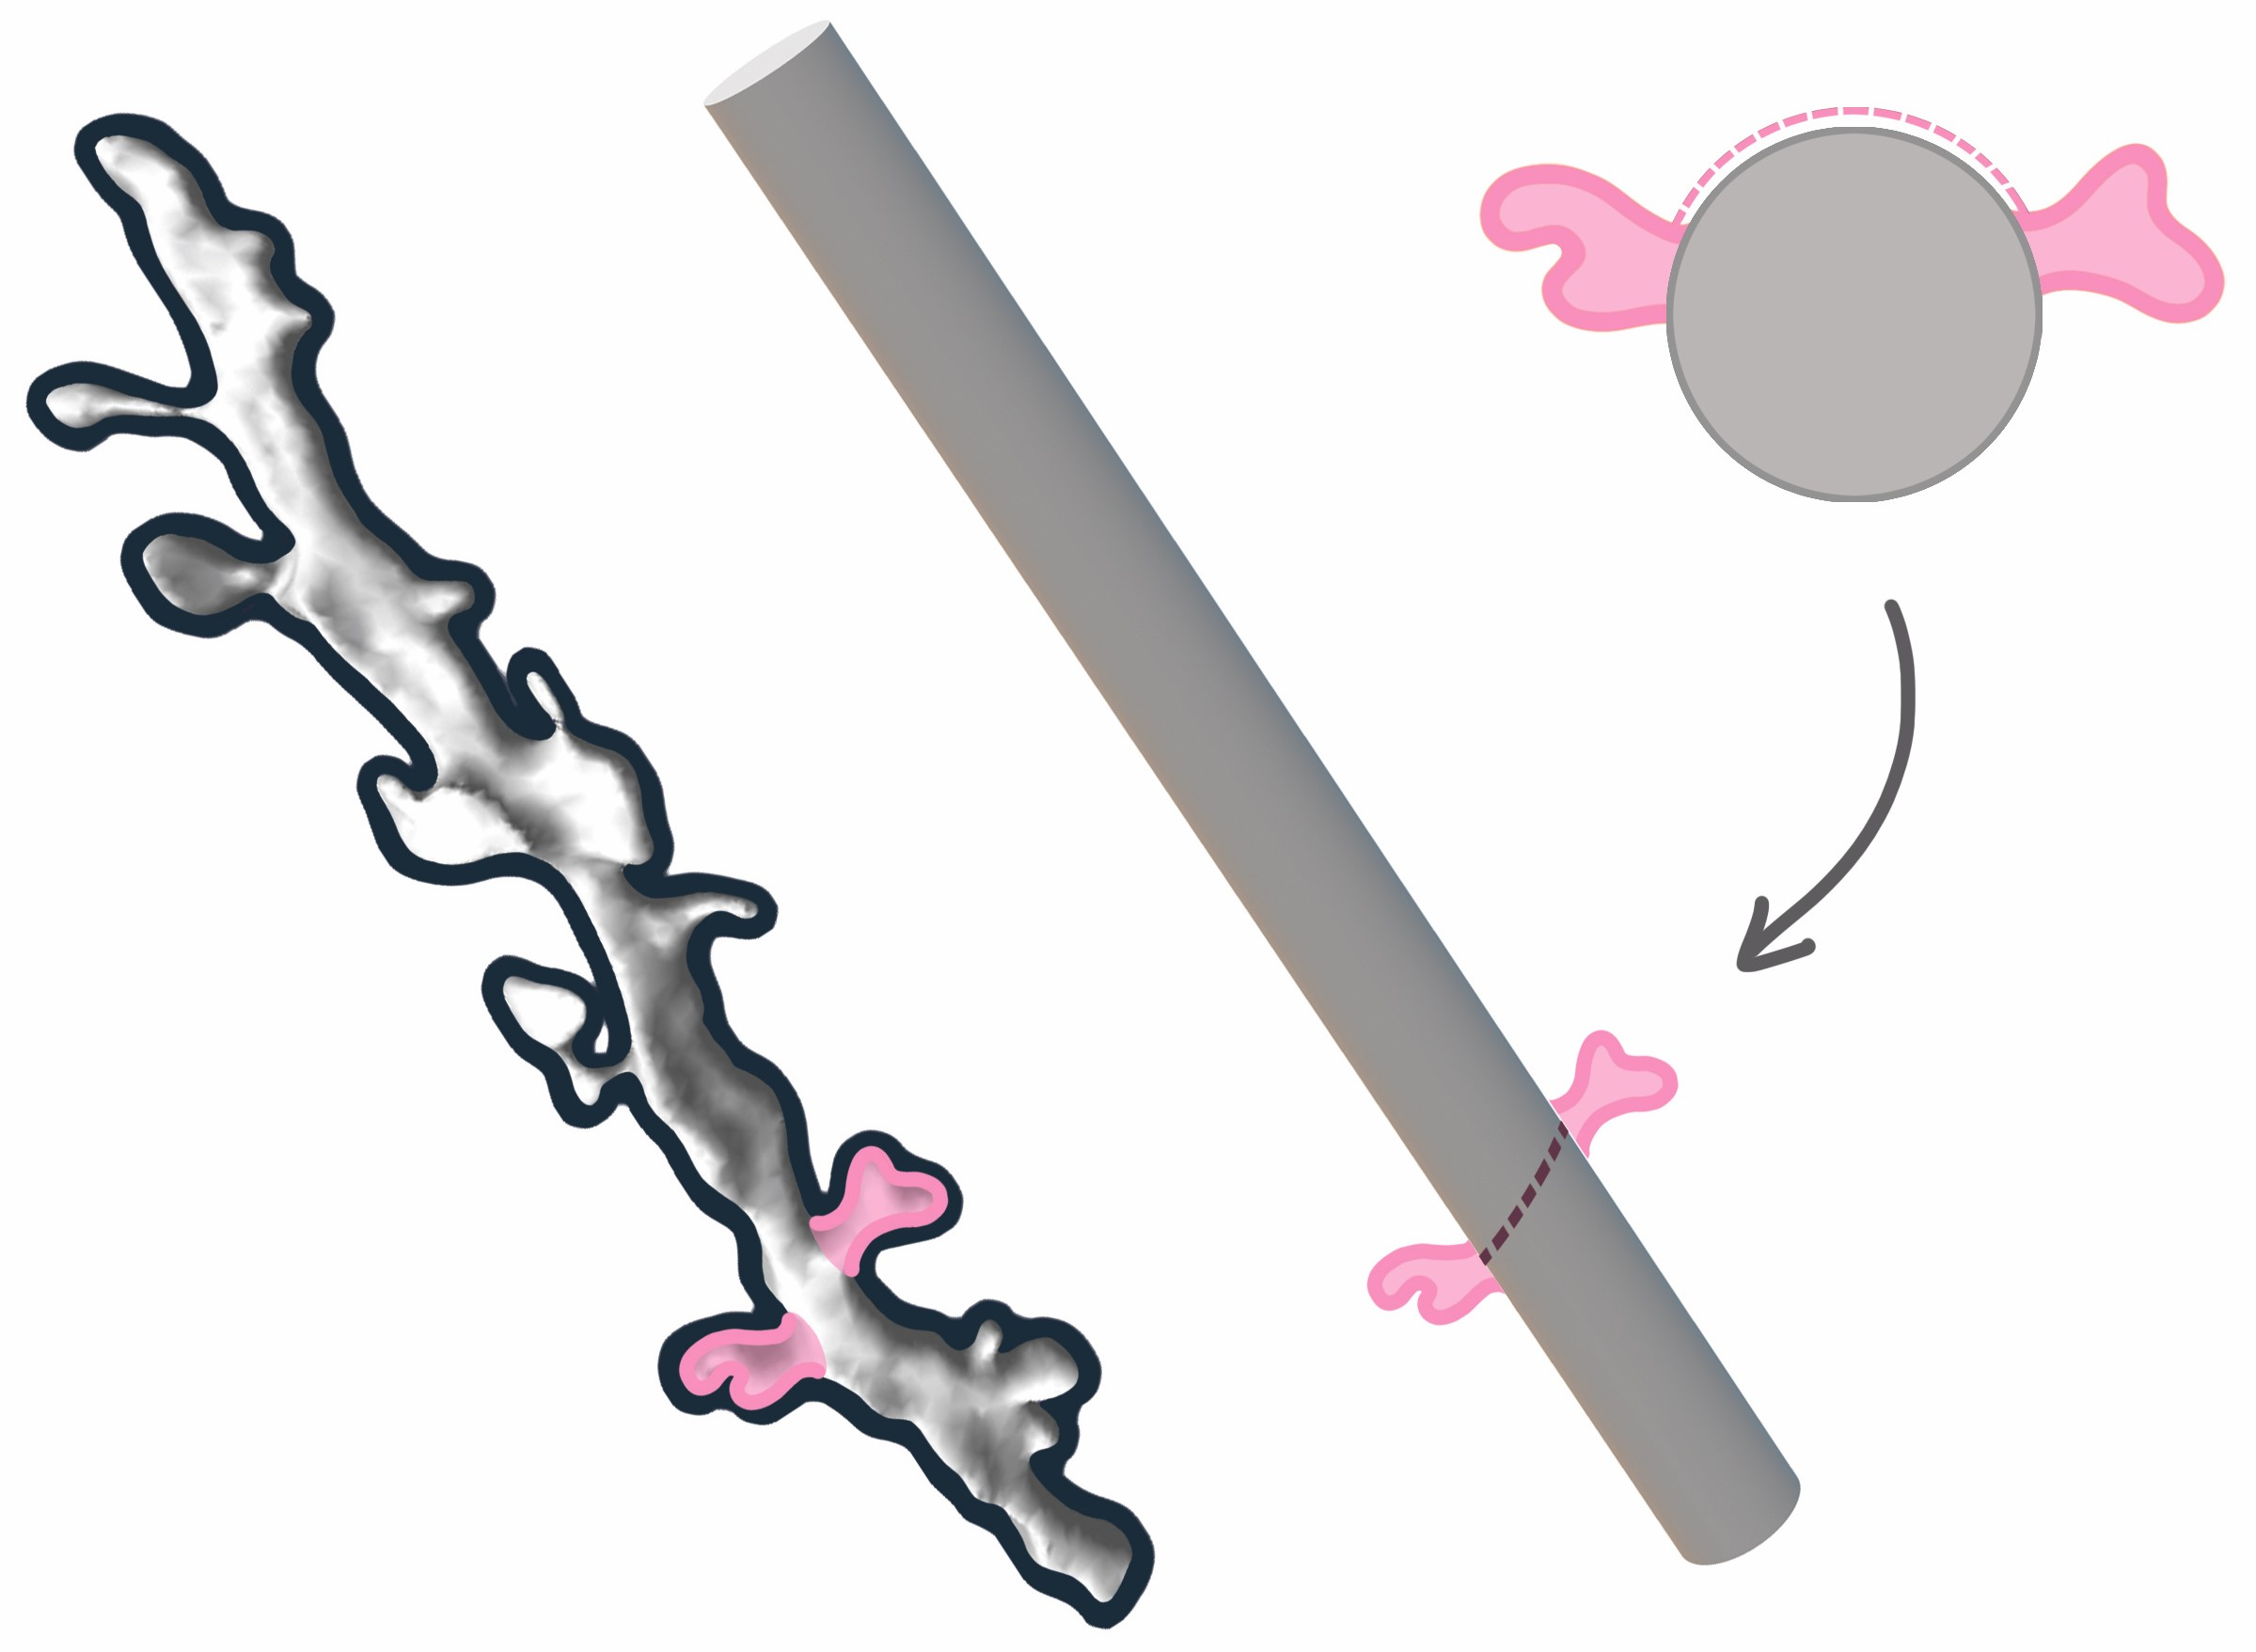
\includegraphics[width=\linewidth]{цк.jpg} % \linewidth = ширина subfigure
    %         \caption{\centering Вычисление расстояния в цилиндрических координатах}
    %         \label{fig:graph1}
    %     \end{subfigure}
    %     \hfill % добавляем промежуток
    %     \begin{subfigure}[b]{0.48\textwidth}
    %         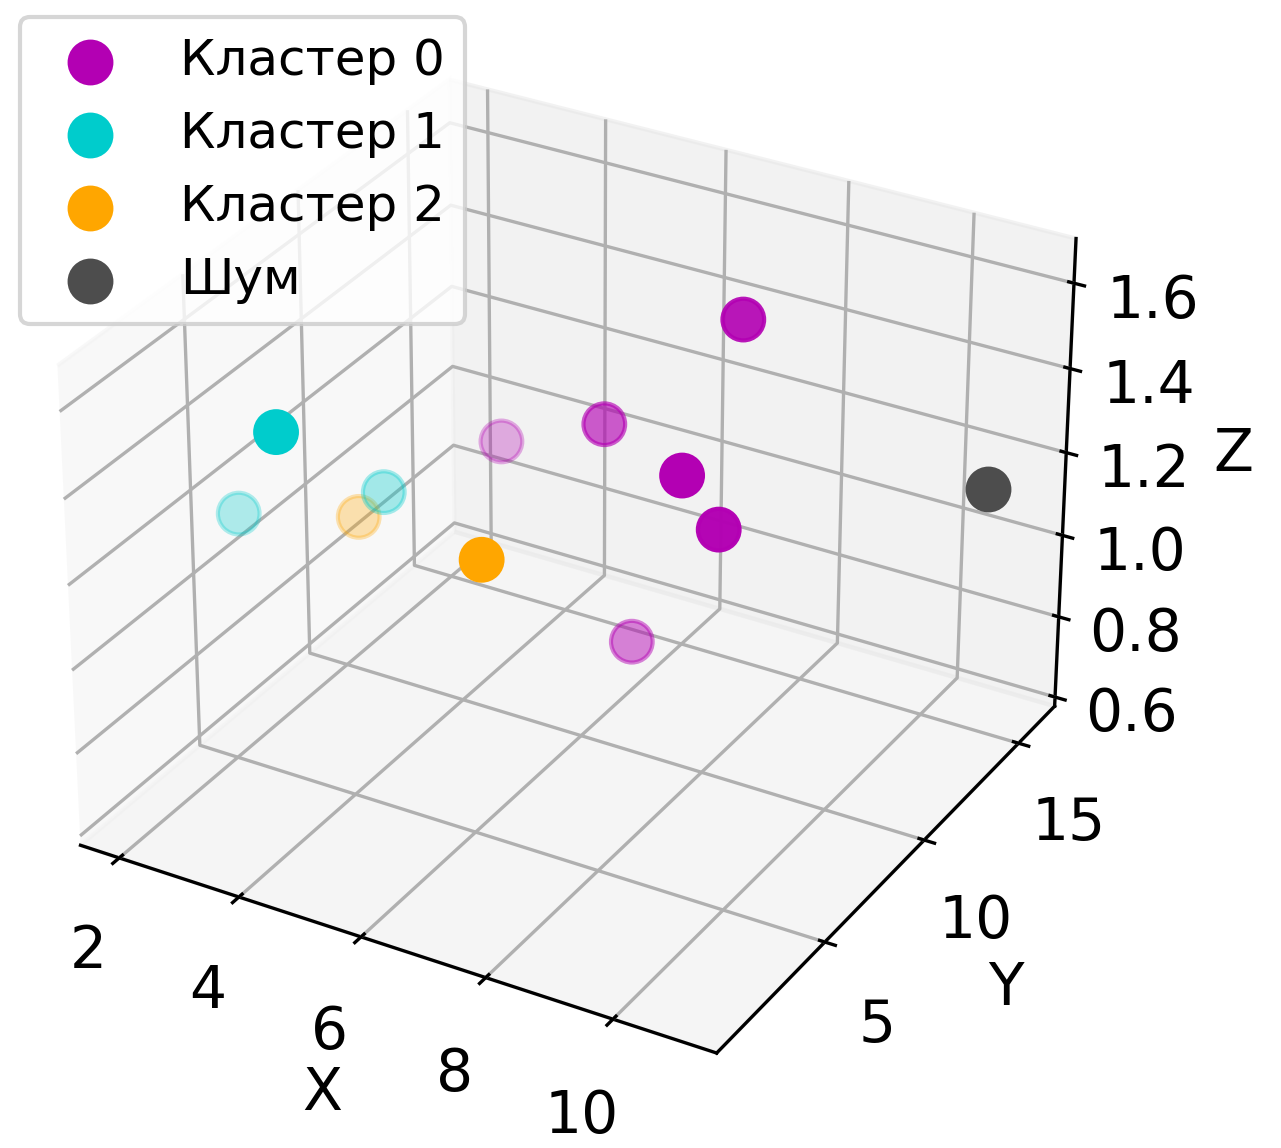
\includegraphics[width=\linewidth]{ab23-2_processed.png}
    %         \caption{Пример результата кластеризации}
    %         \label{fig:graph2}
    %     \end{subfigure}
    %     % \caption{Общая подпись (опционально)} % можно убрать, если не нужно
    %     \label{fig:both}
    % \end{figure}
    % \vspace{-0.7em}
    % \vspace{-0.6em}
    \begin{figure}[ht]
    \centering
    \begin{minipage}[t]{0.48\textwidth}
        \centering
        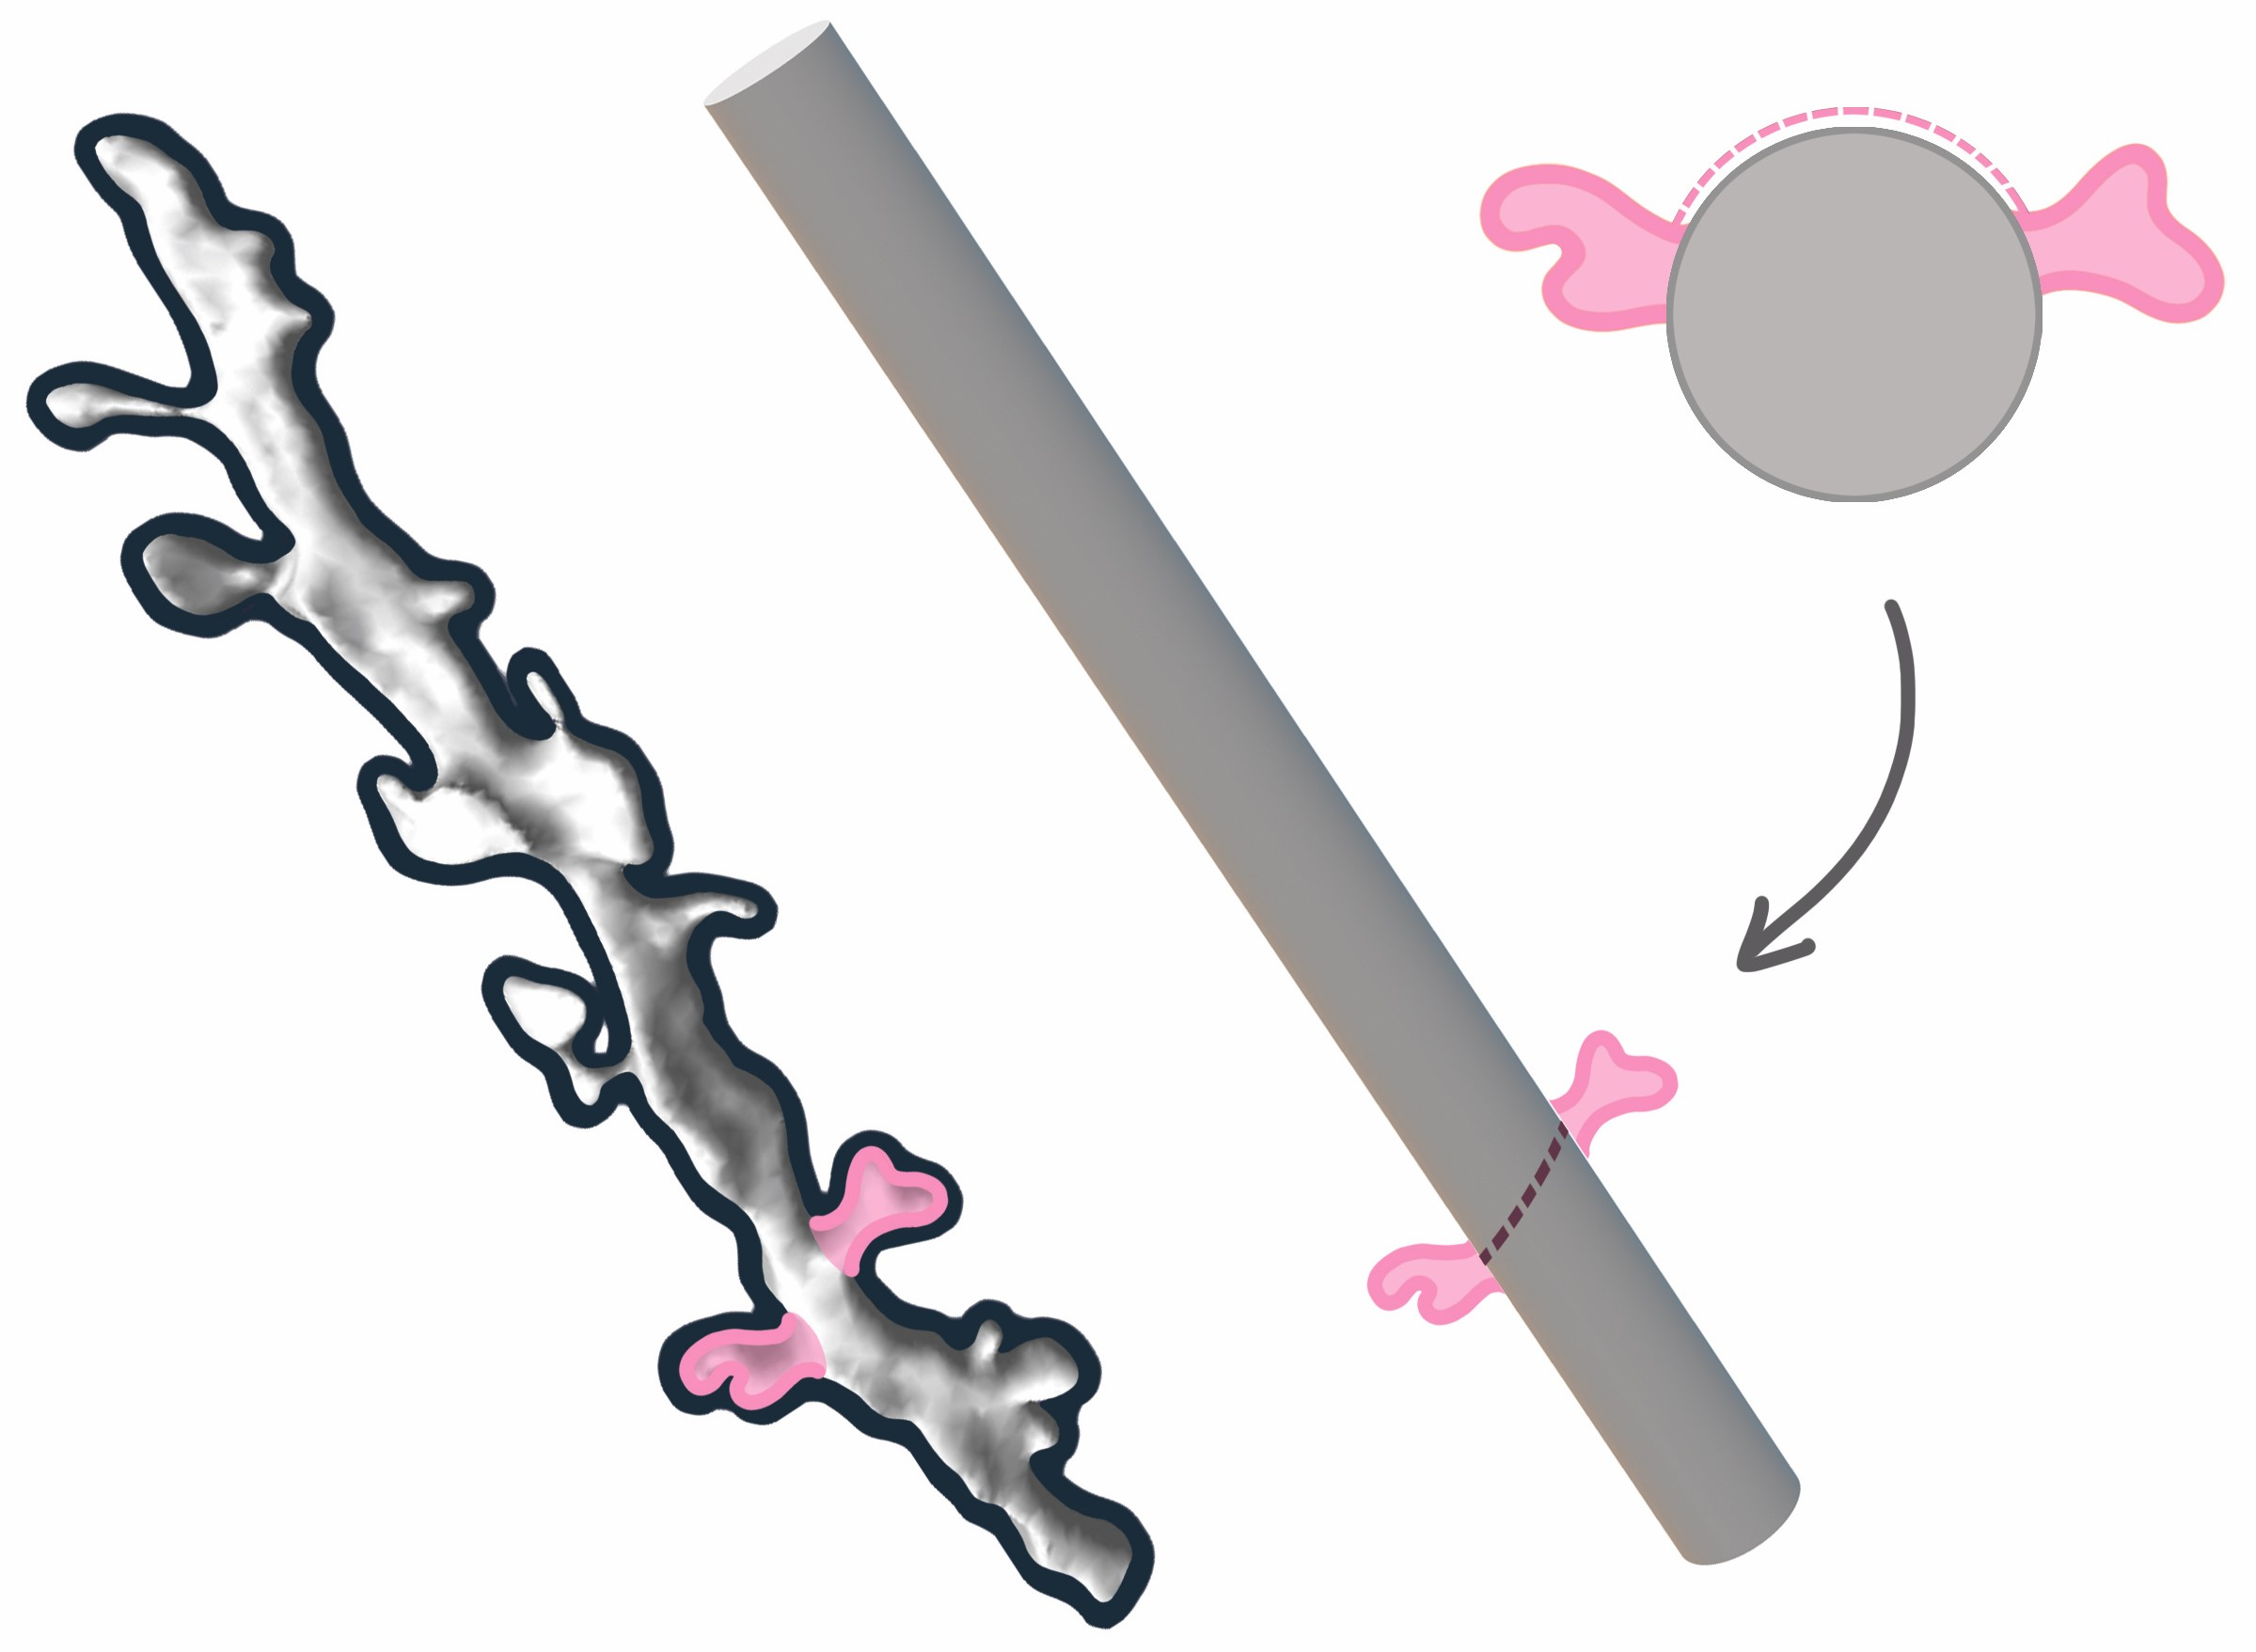
\includegraphics[width=\linewidth]{цк.jpg}
        \caption{\centering Вычисление расстояния в цилиндрических координатах}
        \label{fig:graph1}
    \end{minipage}
    \hfill
    \begin{minipage}[t]{0.48\textwidth}
        \centering
        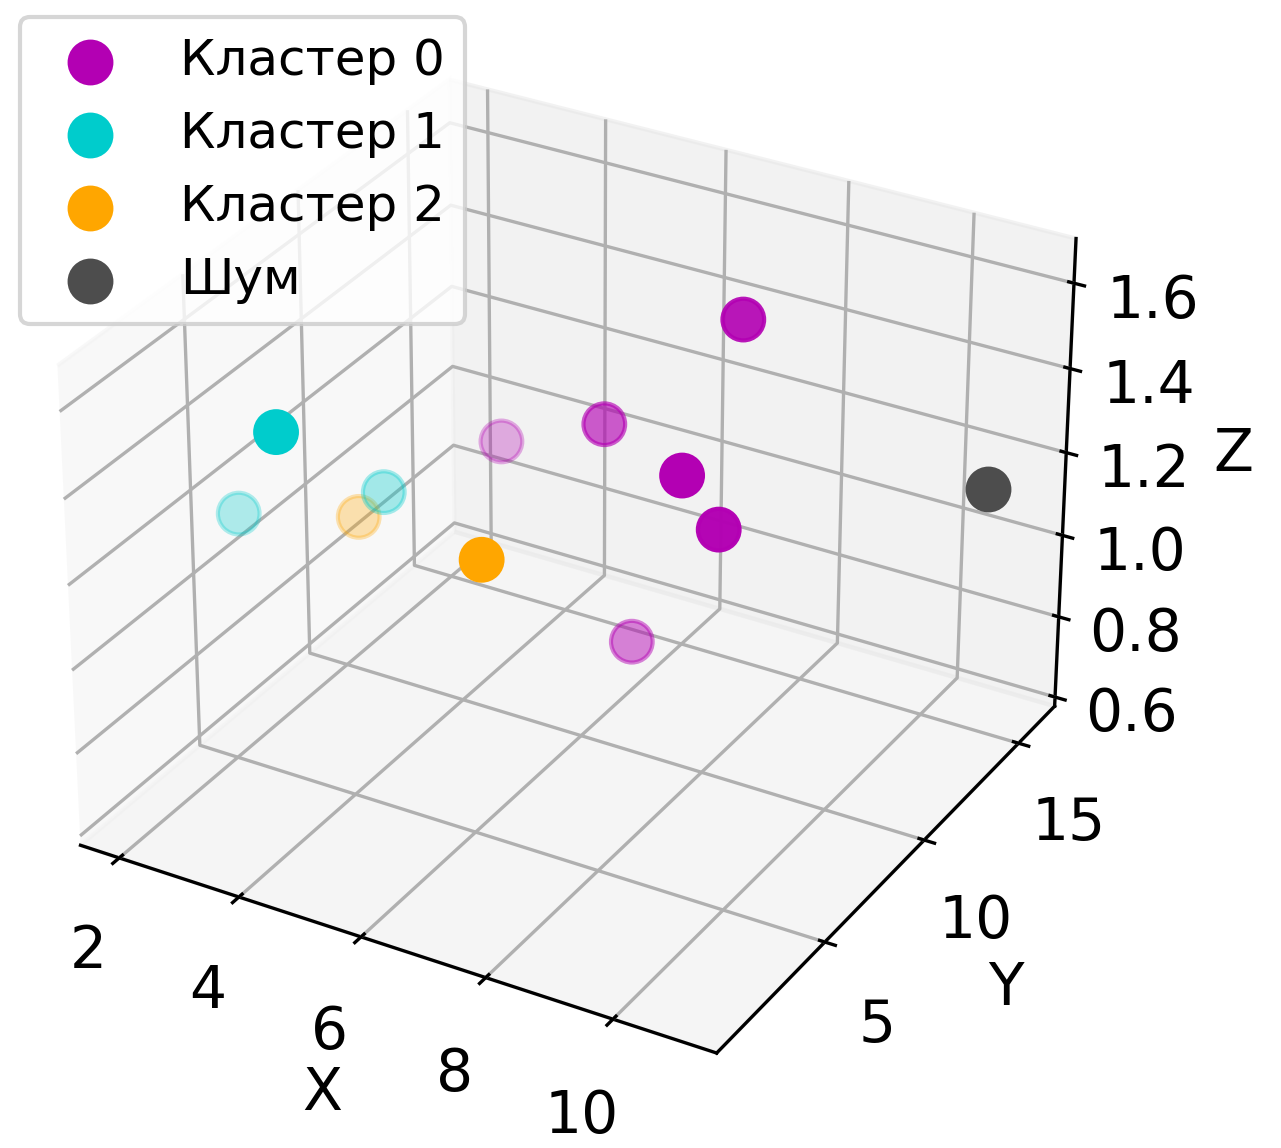
\includegraphics[width=\linewidth]{ab23-2_processed.png}
        \caption{Пример результата кластеризации}
        \label{fig:graph2}
    \end{minipage}
    \end{figure}

    % \begin{itemize}
    %   \item \textbf{Анализ распределения попарных расстояний между шипиками} 
    %   \item \textbf{Вычисление метрики NNdist: } 
    %   $$ NNdist = \frac {1} {n} \sum\limits_{i=1}^n \min\limits_{i \neq j}⁡ dist(p_i,p_j ) $$
    %   где $p_i$ – некоторая точка, $p_j$ – ближайший сосед $p_i$. 
    %   \item \textbf{Вычисление функции парной корреляции PCF: } 
    %   $$g(r)= \frac {\rho(r)} {\rho_0} $$
    %   где $\rho(r)$ – средняя плотность точек на расстоянии $r$ от некоторой точки, $\rho_0$ – средняя плотность точек.
    %   \item \textbf{Вычисление энтропии Шеннона: } 
    %   $$ S= -\sum\limits_{i=1}^n p(r_i) \cdot \log⁡ p(r_i) $$
    %   \item \textbf{Вычисление меры автокорреляции Морана} morbi justo neque, ullamcorper
    %   \item \textbf{Анализ пространственных кластеров} morbi justo neque, ullamcorper
    % \end{itemize}

    % Eget augue porta, bibendum venenatis tortor.

  \end{block}
  
  \vspace{-0.8em}  
  
  \begin{block}{Описание эксперимента}
    Набор данных состоял из 60 дендритов первичных гиппокомпальных нейронов, 616 дендритных шипиков, извлеченных из микроскопических снимков с помощью программного обеспечения SpineTool [1]:\\
    % \vspace{-0.7em}
    \begin{itemize}
      \item дендриты мышей дикого типа (Wt)
      \item дендриты обработанные олигомерной формой бетта-амилоида 42 (Ab), моделирующие болезнь Альцгеймера.
    \end{itemize}

  % Для проведения анализа использовались данные двух групп дендритов:
  % Данные культур:
  % \vspace{-0.7em}
  % \begin{itemize}
  %     \item Wt - дендриты культуры гиппокампа мышей дикого типа, 37 дендритов
  %     \item Ab - дендриты культуры моделирующие болезнь Альцгеймера, 24 дендрита
  % \end{itemize}
    Для выявления отличий между распределениями значений метрик дендритов типа Wt и Ab был выполнен двухвыборочный тест Колмогорова-Смирнова (табл. 1) и построено графическое отображение распределений (рис. 5, 6).

  \end{block}

  % \begin{alertblock}{A highlighted block}

  %   This block catches your eye, so \textbf{important stuff} should probably go
  %   here.

  %   Curabitur eu libero vehicula, cursus est fringilla, luctus est. Morbi
  %   consectetur mauris quam, at finibus elit auctor ac. Aliquam erat volutpat.
  %   Aenean at nisl ut ex ullamcorper eleifend et eu augue. Aenean quis velit
  %   tristique odio convallis ultrices a ac odio.

  %   \begin{itemize}
  %     \item \textbf{Fusce dapibus tellus} vel tellus semper finibus. In
  %       consequat, nibh sed mattis luctus, augue diam fermentum lectus.
  %     \item \textbf{In euismod erat metus} non ex. Vestibulum luctus augue in
  %       mi condimentum, at sollicitudin lorem viverra.
  %     \item \textbf{Suspendisse vulputate} mauris vel placerat consectetur.
  %       Mauris semper, purus ac hendrerit molestie, elit mi dignissim odio, in
  %       suscipit felis sapien vel ex.
  %   \end{itemize}

  %   Aenean tincidunt risus eros, at gravida lorem sagittis vel. Vestibulum ante
  %   ipsum primis in faucibus orci luctus et ultrices posuere cubilia Curae.

  % \end{alertblock}

%  \begin{block}{Nullam vel erat at velit convallis laoreet}

%     Class aptent taciti sociosqu ad litora torquent per conubia nostra, per
%     inceptos himenaeos. Phasellus libero enim, gravida sed erat sit amet,
%     scelerisque congue diam. Fusce dapibus dui ut augue pulvinar iaculis.



%     Donec quis posuere ligula. Nunc feugiat elit a mi malesuada consequat. Sed
%     imperdiet augue ac nibh aliquet tristique. Aenean eu tortor vulputate,
%     eleifend lorem in, dictum urna. Proin auctor ante in augue tincidunt
%     tempor. Proin pellentesque vulputate odio, ac gravida nulla posuere
%     efficitur. Aenean at velit vel dolor blandit molestie. Mauris laoreet
%     commodo quam, non luctus nibh ullamcorper in. Class aptent taciti sociosqu
%     ad litora torquent per conubia nostra, per inceptos himenaeos.

%     Nulla varius finibus volutpat. Mauris molestie lorem tincidunt, iaculis
%     libero at, gravida ante. Phasellus at felis eu neque suscipit suscipit.
%     Integer ullamcorper, dui nec pretium ornare, urna dolor consequat libero,
%     in feugiat elit lorem euismod lacus. Pellentesque sit amet dolor mollis,
%     auctor urna non, tempus sem.

%   \end{block}

\end{column}

\separatorcolumn

\begin{column}{\colwidth}

  \begin{block}{Результаты}

    Результаты теста Колмогорова-Смирнова для распределения попарных расстояний (рис. 4) между шипиками показали статистическую значимость разницы распределений для Wt и Ab. 
    % \vspace{-0.7em} 
    \begin{figure}
        \centering
        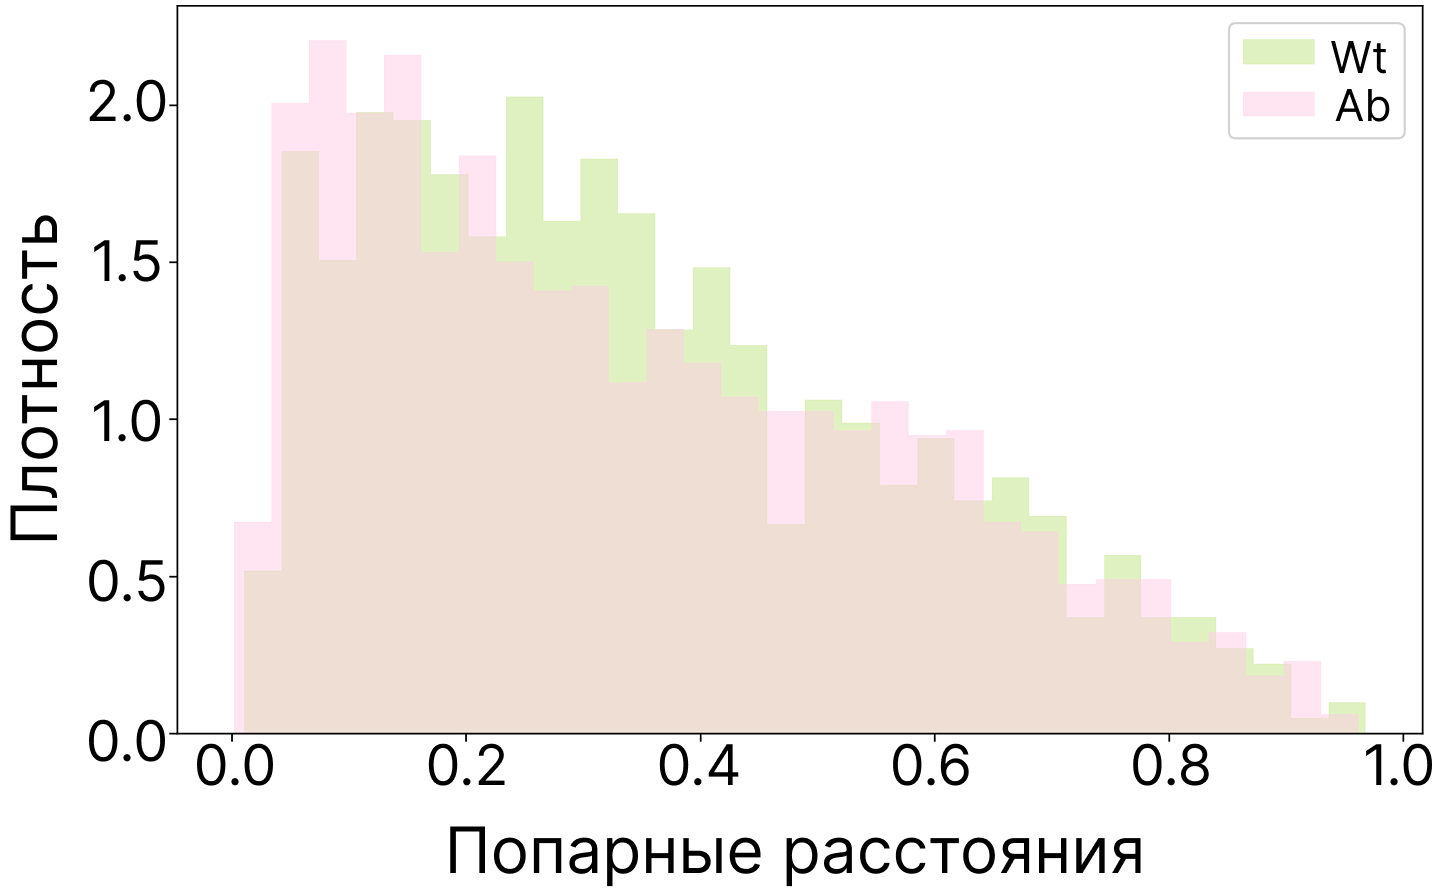
\includegraphics[width=0.5\linewidth]{distribution_figma.png}
        \caption{Распределение попарных расстояний между шипиками}
        \label{fig:enter-label}
    \end{figure}
    % \vspace{-0.9em} 
    % \begin{figure}
    %     \centering
    %     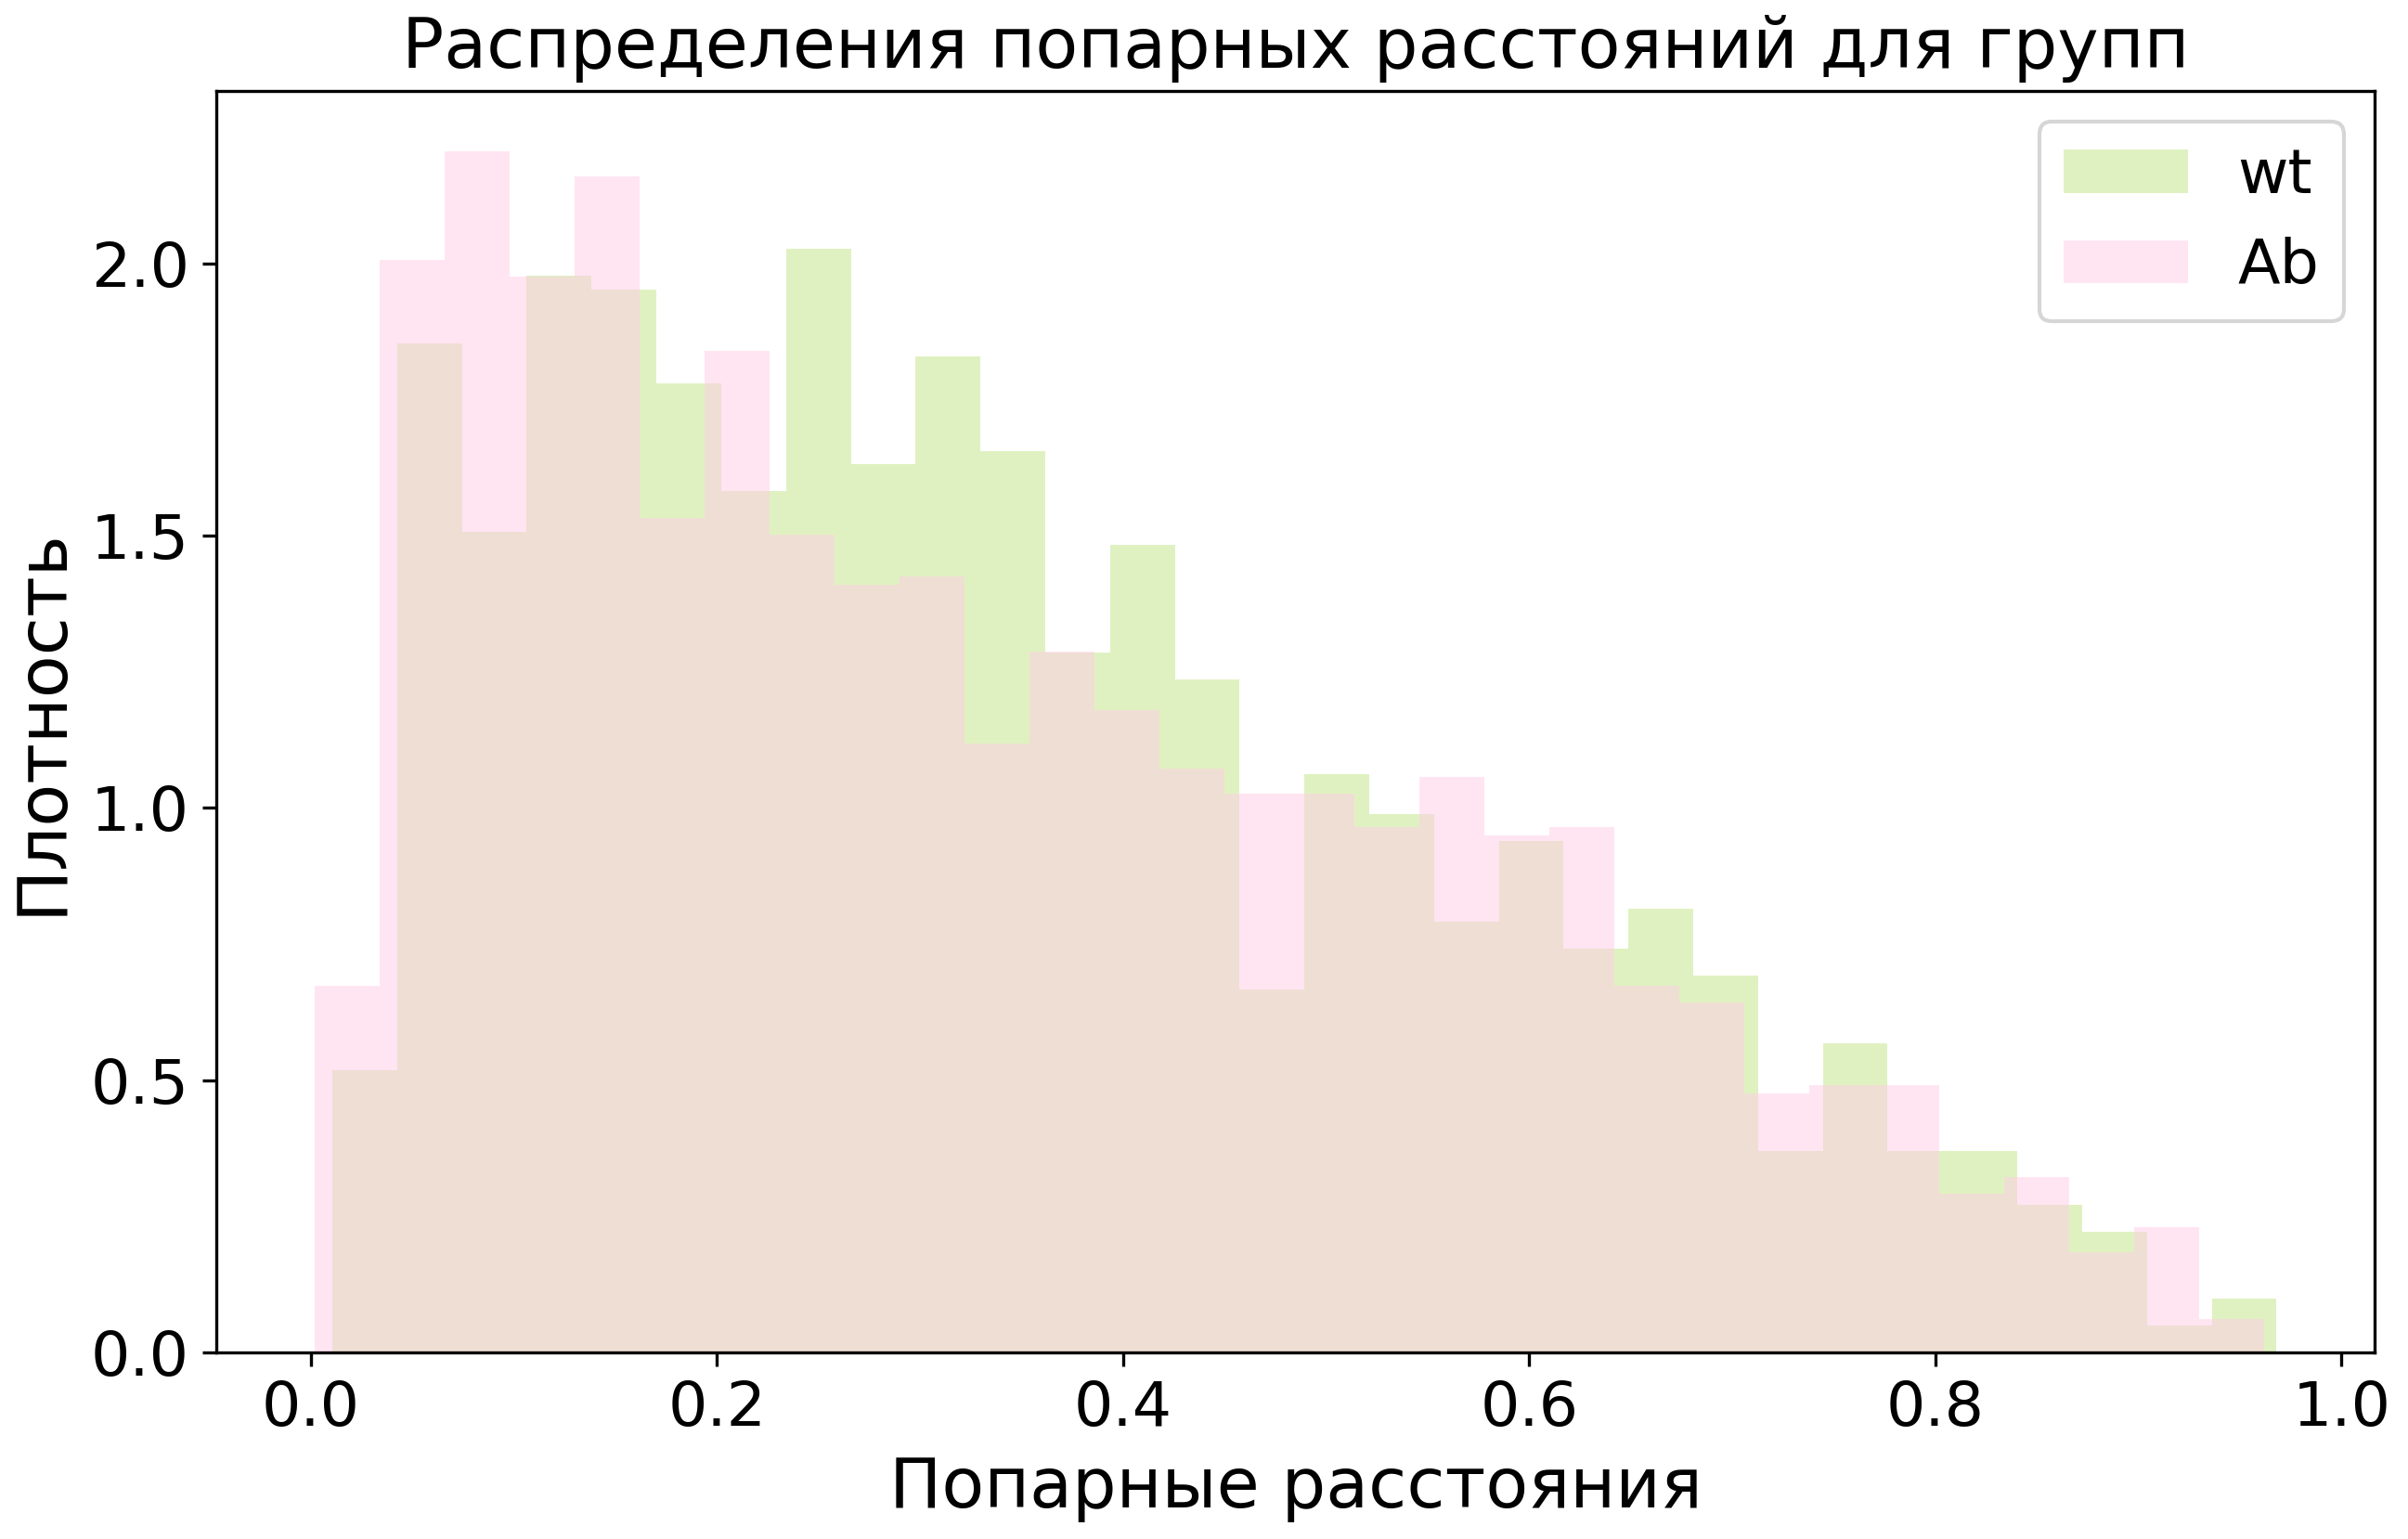
\includegraphics[width=0.5\linewidth]{distribution.png}
    %     \caption{Распределение попарных расстояний между шипиками}
    %     \label{fig:enter-label}
    % \end{figure}
    % \vspace{-0.8em}  

  \begin{table}[!htb]
      \centering
      \renewcommand{\arraystretch}{1.3} %% increase table row spacing
      % \renewcommand{\tabcolsep}{0.4cm}
      % \begin{tabular}{|l|r|r|r|r|}
      \begin{tabular}{|c|c|c|c|c|}
        \hline
        \rowcolor{mycolor1}& \multicolumn{2}{i|}{\textbf{Среднее значение}} & \multicolumn{2}{i|}{\textbf{Тест КС}} \\
        \cline{2-5}
        \rowcolor{mycolor1}\raisebox{1.5ex}[0cm][0cm]{\textbf{Метрика}} & \textbf{Ab} & \textbf{Wt} & \textbf{Статистика} & \textbf{p-value} \\ \hline
        NNdist & 2.31 & 2.25 & 0.18 & 0.652 \\
        Энтропия Шеннона & 2.73 & 3.37 & 0.48 & 0.001 \\
        Мера Морана метрики «Объем» & -0.03 & -0.16 & 0.43 & 0.008 \\
        $\varepsilon$ & 2.56 & 3.08 & 0.19 & 0.577 \\
        m & 1.94 & 2.10 & 0.16 & 0.778 \\
        Статистика теста Крускала-Уоллиса & 2.44 & 974 & 0.25 & 0.270 \\
        p-value теста Крускала-Уоллиса & 0.20 & 0.32 & 0.57 & 6.741 \\
        Доля шума & 0.14 & 0.21 & 0.33 & 0.600 \\ \hline
      \end{tabular}
      \caption{Средние значения метрик и результаты теста Колмогорова-Смирнова}
  \end{table}
  \vspace{-0.7em} 

%   \begin{table}[!htb]
%     \centering
%     \renewcommand{\arraystretch}{1.3}
%     \begin{tabular}{|c|c|c|c|c|}
%         \hline
%         \rowcolor{blue!10}& \multicolumn{2}{c|}{\textbf{Среднее значение}} & \multicolumn{2}{c|}{\textbf{Тест КС}} \\
%         \cline{2-5}
%         \rowcolor{blue!10}\raisebox{1.5ex}[0cm][0cm]{\textbf{Метрика}} & \textbf{Ab} & \textbf{Wt} & \textbf{Статистика} & \textbf{p-value} \\ \hline
%         \rowcolor{blue!10} NNdist & 2.31 & 2.25 & 0.18 & 0.652 \\
%         \rowcolor{green!10} Энтропия Шеннона & 2.73 & 3.37 & 0.48 & 0.001 \\
%         \rowcolor{blue!10} Мера Морана метрики «Объем» & -0.03 & -0.16 & 0.43 & 0.008 \\
%         \rowcolor{green!10} $\varepsilon$ & 2.56 & 3.08 & 0.19 & 0.577 \\
%         \rowcolor{blue!10} m & 1.94 & 2.10 & 0.16 & 0.778 \\
%         \rowcolor{green!10} Статистика теста Крускала-Уоллиса & 2.44 & 974 & 0.25 & 0.270 \\
%         \rowcolor{blue!10} p-value теста Крускала-Уоллиса & 0.20 & 0.32 & 0.57 & 6.741 \\
%         \rowcolor{green!10} Доля шума & 0.14 & 0.21 & 0.33 & 0.600 \\ \hline
%     \end{tabular}
%     \caption{Средние значения метрик и результаты теста Колмогорова-Смирнова}
% \end{table}

    \begin{figure}
        \centering
        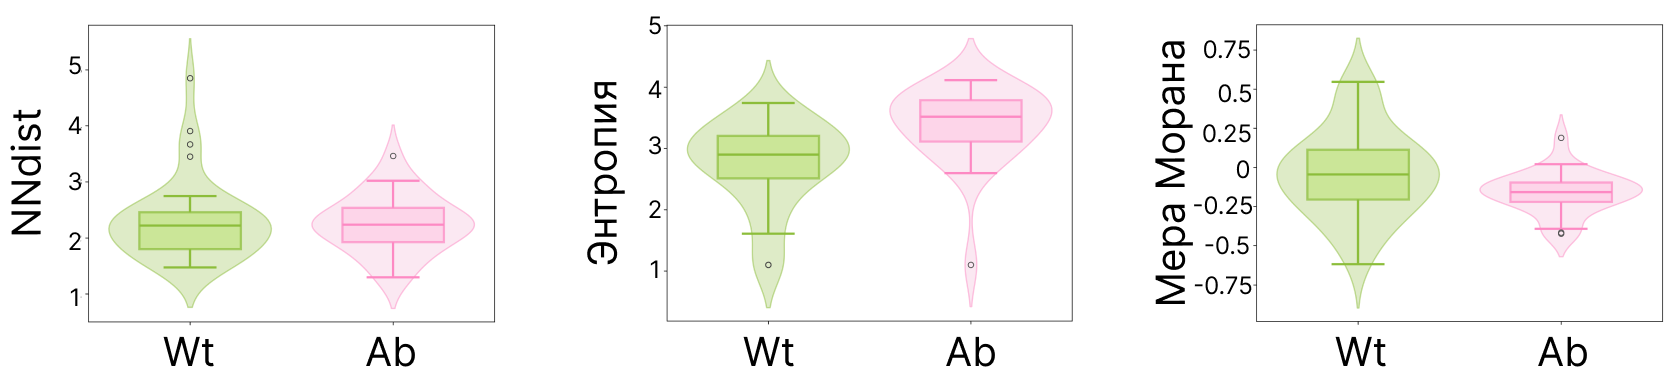
\includegraphics[width=1\linewidth]{базовые метрики.png}
        \caption{\centering Статистическое распределение значений метрик пространственной структурированности}
        \label{fig:enter-label}
    \end{figure}
    \vspace{-0.7em} 

    \begin{figure}
        \centering
        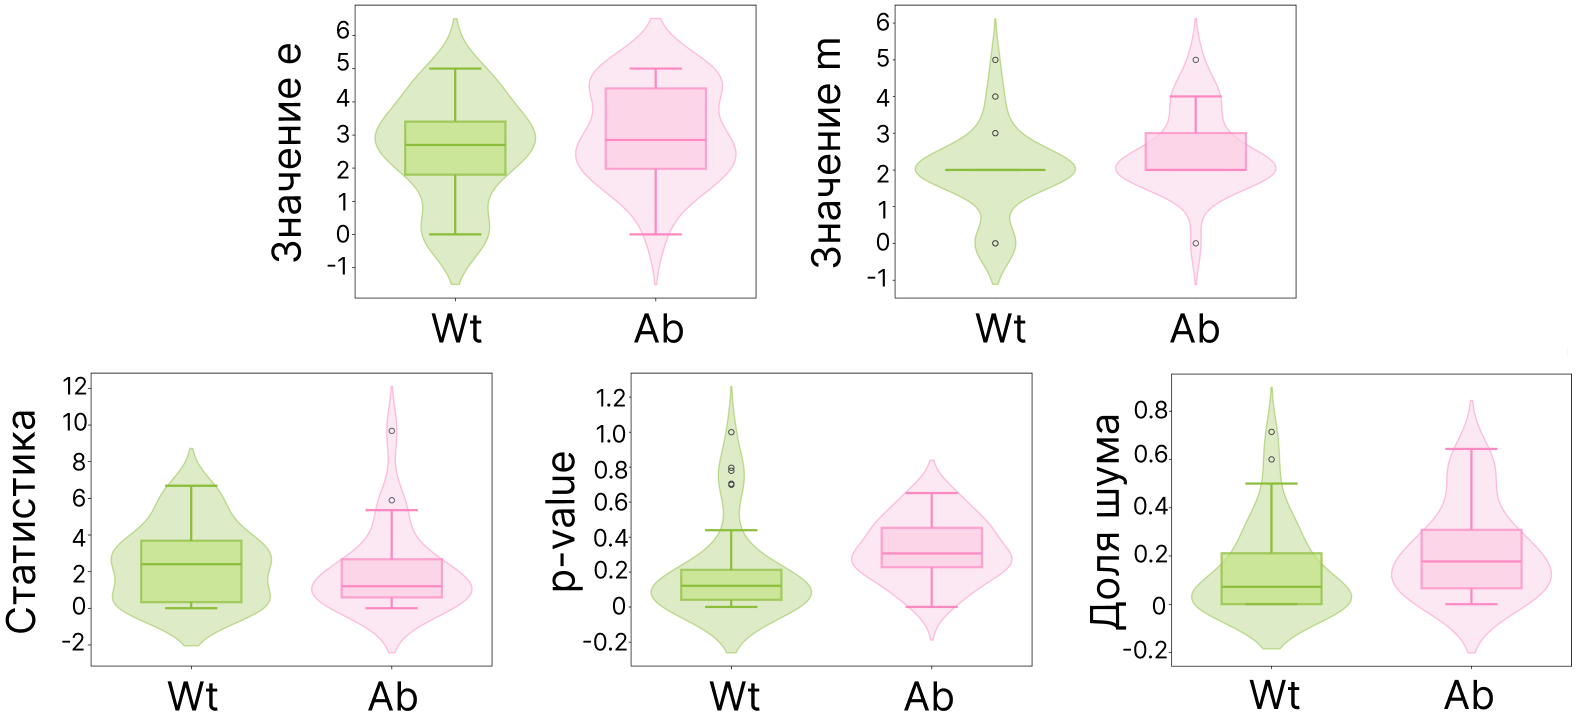
\includegraphics[width=1\linewidth]{оптимальные парметры DBSCAN.png}
        \caption{Статистическое распределение метрик кластеризуемости}
        \label{fig:enter-label}
    \end{figure}
    \vspace{-0.95em} 

    \heading{Выводы:}
    \begin{itemize}
        \item \textbf{NNdist:} статистически значимых отличий нет.
        \item \textbf{PCF:} для Ab значение PCF выше, чем для Wt, отличия статистически значимы, что свидетельствует о наличии более выраженной структуры дендрита.
        \item \textbf{Мера Морана:} для Ab наблюдается статистически значимое уменьшение значений метрики, следовательно при патологии наблюдается более выраженная отрицательная автокорреляция относительно объема. 
        \item \textbf{Параметры кластеризации:} статистически значимых отличий нет. 
        \item \textbf{Доля шума:} у Ab выше, чем у Wt, отличия статистически значимы, следовательно, у Ab шипики склонны вырастать вне окрестностей шипиков.
    \end{itemize}

  \end{block}
  % \vspace{-0.8em} 

  Настоящее исследование было поддержано грантом в рамках государственного задания FSEG-2024-0025 и Фондом поддержки инноваций и молодежных инициатив Санкт-Петербурга в рамках проекта «Кампус цифровых лабораторий Blue Sky Research».

  % \begin{block}{Заключение}

  %   В ходе анализа взаимного расположения дендритных шипиков в норме и при нейродегенерации были выявлены отличительные особенности дендритов рассмотренных типов: диких мышей и модели Альцгеймера. Кроме того, были выявлены метрики, которые остаются неизменными в случае нейропаталогии. 

  % \end{block}

  % \begin{block}{Nam cursus consequat egestas}

  %   Etiam sit amet tempus lorem, aliquet condimentum velit. Donec et nibh
  %   consequat, sagittis ex eget, dictum orci. Etiam quis semper ante. Ut eu
  %   mauris purus. Proin nec consectetur ligula. Mauris pretium molestie
  %   ullamcorper. Integer nisi neque, aliquet et odio non, sagittis porta justo.

  %   \begin{itemize}
  %     \item \textbf{Sed consequat} id ante vel efficitur. Praesent congue massa
  %       sed est scelerisque, elementum mollis augue iaculis.
  %       \begin{itemize}
  %         \item In sed est finibus, vulputate
  %           nunc gravida, pulvinar lorem. In maximus nunc dolor, sed auctor eros
  %           porttitor quis.
  %         \item Fusce ornare dignissim nisi. Nam sit amet risus vel lacus
  %           tempor tincidunt eu a arcu.
  %         \item Donec rhoncus vestibulum erat, quis aliquam leo
  %           gravida egestas.
  %       \end{itemize}
  %     \item \textbf{Pellentesque facilisis dolor in leo} bibendum congue.
  %       Maecenas congue finibus justo, vitae eleifend urna facilisis at.
  %   \end{itemize}

  % \end{block}

 

  \begin{block}{Литература}
      [1] Pchitskaya E. et al. SpineTool is an open-source software for analysis of morphology of dendritic spines //Scientific reports. – 2023. – Т. 13. – №. 1. – С. 10561. \\
    % [1] Penzes P. et al. Dendritic spine pathology in neuropsychiatric disorders //Nature neuroscience. – 2011. – Т. 14. – №. 3. – С. 285-293. \\
    % [2] Frank A. C. et al. Hotspots of dendritic spine turnover facilitate clustered spine addition and learning and memory //Nature communications. – 2018. – Т. 9. – №. 1. – С. 422. \\
    % [3] Pchitskaya E. et al. SpineTool is an open-source software for analysis of morphology of dendritic spines //Scientific reports. – 2023. – Т. 13. – №. 1. – С. 10561. \\
    % [4]. Ilamathi H. S. et al. Mitochondrial fission is required for proper nucleoid distribution within mitochondrial networks //bioRxiv. – 2021. – С. 2021.03. 17.435804. \\
    % [5] Toffin E. et al. Colonization of weakened trees by mass-attacking bark beetles: No penalty for pioneers, scattered initial distributions and final regular patterns //Royal Society open science. – 2018. – Т. 5. – №. 1. – С. 170454. \\
    % [6]. Ilamathi H. S. et al. A new automated tool to quantify nucleoid distribution within mitochondrial networks //Scientific reports. – 2021. – Т. 11. – №. 1. – С. 22755. \\
    % [7] Chen Y. An analytical process of spatial autocorrelation functions based on Moran’s index //PLoS One. – 2021. – Т. 16. – №. 4. – С. e0249589. \\
    % [8] Deng D. DBSCAN clustering algorithm based on density //2020 7th international forum on electrical engineering and automation (IFEEA). – IEEE, 2020. – С. 949-953. \\
    % [9] Ostertagova E., Ostertag O., Kováč J. Methodology and application of the Kruskal-Wallis test //Applied mechanics and materials. – 2014. – Т. 611. – С. 115-120. \\

  %   % \nocite{*}
  %   % \footnotesize{\bibliographystyle{plain}\bibliography{poster}}

  \end{block}

\end{column}
\separatorcolumn



\end{columns}
\end{frame}

\end{document}
